\documentclass[12pt]{article}
\usepackage[utf8]{inputenc}
\usepackage[T1]{fontenc}
\usepackage{mathptmx}
\usepackage{geometry}
\usepackage{mathtools}
\usepackage[english]{babel}
\usepackage{graphicx}
\usepackage[figurename=Gambar]{caption}
\usepackage{hyperref}
\usepackage{minted}
\usepackage{setspace}
\usepackage{color}
\usepackage[explicit]{titlesec}
\usepackage{tocloft}
\usepackage{titletoc}
\usepackage{indentfirst}
\usepackage{caption}
\usepackage{subcaption}
\usepackage{amsmath} 
\usepackage{pdfpages}

%\color{white}
%\pagecolor{black}

\hypersetup{colorlinks,
	citecolor=black,
	filecolor=black,
	linkcolor=black,
	urlcolor=black
}

\geometry{
	a4paper,
	left=40mm,
	right=30mm,
	top=20mm,
	bottom=20mm,
}

\date{}

%=============================================================================
% Modified Items

\providecommand{\keywordid}[1]{\textit{Kata Kunci: } #1}
\providecommand{\keyworden}[1]{\textit{Keywords: } #1}

\titleformat{\section}{}{}{0pt}{}
\titleformat{\subsubsection}{\small \bfseries}{\thesubsection}{0pt}{}

\renewcommand{\cftsecleader}{\cftdotfill{\cftdotsep}}
\renewcommand{\cftsubsecleader}{\cftdotfill{\cftdotsep}}

\makeatletter
\let\latexl@section\l@section
\def\l@section#1#2{\begingroup\let\numberline\@gobble\latexl@section{#1}{#2}\endgroup}
\makeatother

\addto\captionsenglish{\renewcommand{\contentsname}{}}
\addto\captionsenglish{\renewcommand{\listfigurename}{}}

\renewcommand{\cftsecfont}{\normalfont}
\renewcommand{\cftsecpagefont}{\normalfont}

\renewcommand{\thefigure}{\arabic{section}.\arabic{figure}}

%=============================================================================
% Document Part

\begin{document}
	
\onehalfspacing

%=============================================================================
% Cover
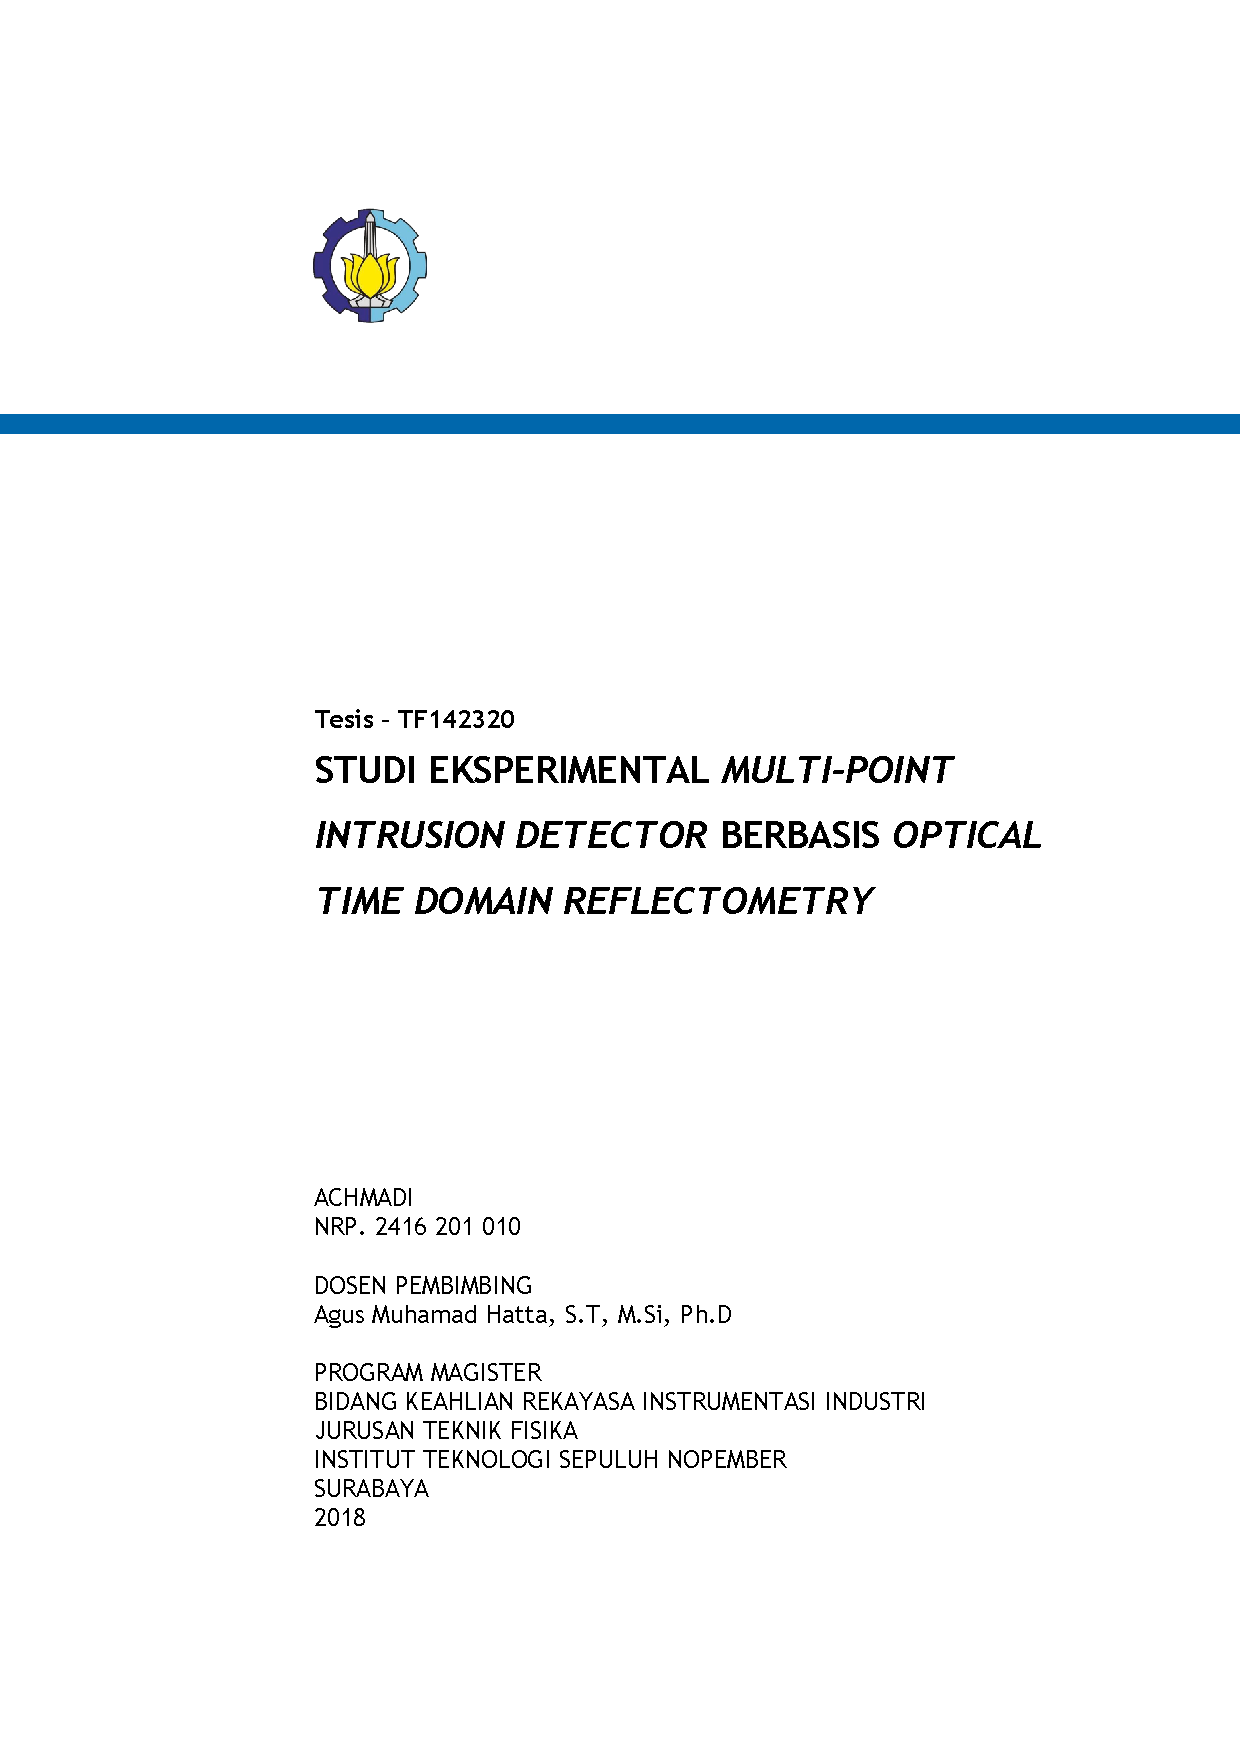
\includepdf[pages=-]{images/cover.pdf}

%=============================================================================
%\newpage
%\thispagestyle{plain}
%\mbox{}

%=============================================================================
% Abstrak Indonesia
	
	\pagenumbering{roman}
	\setcounter{page}{2}
	
	\section{Abstrak}
	
	\begin{center}
		\large{\textbf{STUDI EKSPERIMENTAL \textit{MULTI-POINT INTRUSION DETECTOR} BERBASIS OPTICAL TIME DOMAIN REFLECTOMETRY}}
	\end{center}

	\vspace{10pt}
	
	\begin{flushleft}
		Nama Mahasiswa : Achmadi \\
		NRP \hspace{62pt}: 24 16 201 010 \\
		Pembimbing \hspace{24pt}: Agus Muhamad Hatta, S.T, M.Si, Ph.D \\
	\end{flushleft}
	
	\vspace{10pt}

	\renewcommand{\abstractname}{ABSTRAK}
	\begin{abstract}
		Penyusup \textit{(intruder/attacker)} merupakan sebuah aktifitas yang tidak bisa dianggap untuk tidak mungkin terjadi apabila berkaitan dengan bangunan, area (perimeter), maupun objek lain dimana memiliki suatu nilai baik militer, ekonomi, maupun industri. 
		Tindak penyusupan memiliki similaritas dengan tindak pencurian dan menjadi awal dari tindak kriminal yang lebih jauh.
		Tindak penyusupan melalui proses melewati sistem pengawasan atau penjagaan.
		Untuk pencegahannya, maka sistem deteksi penyusup telah menjadi bagian penting dalam banyak sistem keamanan.
		Dibutuhkan sistem deteksi yang akurat dan respon yang cepat. Serat optik telah dikenal mampu menjadi transmisi data maupun sebagai sensor.
		Serat optik dapat digunakan sebagai distributed sensor yang mampu menggantikan banyak sensor tipe titik.
		OTDR telah dikenal sebagai salah satu metode karakteriasi serat optik.
		Melalui OTDR akan didapatkan events yang terjadi pada serat optik secara \textit{real-time}.
		Hasil \textit{trace} OTDR dapat digunakan untuk deteksi penyusup.
		Penelitian ini bertujuan untuk merancang sistem deteksi penyusup menggunakan serat optik dan OTDR yang mampu menemukan penyusup dalam multi-point.
		Dalam penelitian ini diusulkan sebuah studi eksperimental untuk mendapatkan rancang bangun sistem sensor terdistribusi berbasis serat optik dan OTDR untuk deteksi penyusup.
		Studi eksperimental disini divariasikan baik konfigurasi serat optik itu sendiri dan juga divariasikan bentuk distribusi sensor.
		Untuk mendapatkan hasil trace maka digunakan modul Mini-OTDR Anritsu MU909015C, sedangkan untuk eksperimen akan dibangun konstruksi pagar yang akan menjadi tempat instalasi sensor.
		Sebagai pengganti tindak intrusi maka diberikan gaya tekan kepada sensor dengan nilai dan jumlah yang telah ditentukan.
		Luaran yang diharapkan dari penelitian ini adalah hasil rancang bangun sensor instrusi terdistribusi dan rancang bangun algoritma untuk mendapatkan posisi multi-point dari tindak intrusi.   
	\end{abstract}

	\keywordid{Serat optik, OTDR, deteksi penyusup, trace, events, sensor terdistribusi}
	
%=============================================================================

\newpage
\thispagestyle{plain}
\mbox{}
	
%=============================================================================
% Abstrak English
	\newpage
	
	\section{Abstract}
	
	\begin{center}
		\large{\textbf{EXPERIMENTAL STUDY OF MULTI-POINT INTRUSION DETECTOR BASED ON OPTICAL TIME DOMAIN REFLECTOMETRY}}
	\end{center}
	
	\vspace{10pt}
	
	\begin{flushleft}
		Nama Mahasiswa : Achmadi \\
		NRP \hspace{62pt}: 24 16 201 010 \\
		Pembimbing \hspace{24pt}: Agus Muhamad Hatta, S.T, M.Si, Ph.D \\
	\end{flushleft}
	
	\vspace{10pt}
	
	\renewcommand{\abstractname}{ABSTRACT}
	\begin{abstract}
		Intrusion by an intruder is an act that cannot be ignored due to a building, an area (perimeter), or any object regarding it’s either milltary, economical, or industrial values.
		Intrusion has high similarity to thieft crime and can be root of more crime act.
		Intrusion is an act that by-passing any survelleince or security system.
		For prevention, a detection system become essential to many security system.
		This detection system has to be highly accurate and fast respons.
		Optical fiber already known for it’s capabilities to both data transmission and as a distributed sensor.
		An distributed sensor mean single optical fiber section can replace many point-type sensors.
		OTDR already known as one of optical fiber characterization.
		Through OTDR, an events that occur on a optical fiber can be aqcuired by real-time.
		An trace result of OTDR can be used to intrusion detector.
		This research purposes is to get designs of an intrusion detector system using optical fiber and OTDR that can detect any multi-point intrusion.
		This research proposed an experimental study to get an intrusion detector using distributed sensor based optical fiber and OTDR.
		This experimental study proposed to test sensor variation in both optical fiber configuration and distributed sensor shape.
		To get trace result, this research use Anritsu MU909015C Mini OTDR module and for experiment, a fence construction is proposed as distributed sensor placement.
		As intrusion act, this research proposed to give a mechanical pressure to sensor with certain amount and magnitude.
		The expected output of this research are design of distributed sensor for intrusion detection and algorithm to get multi-point intrusion positions.
	\end{abstract}
	
	\keyworden{optical fiber, OTDR, instrusion detection, trace, events, distributed sensor}
	
%=============================================================================

\newpage
\thispagestyle{plain}
\mbox{}

%=============================================================================
% Halaman Pengesahan

\newpage

	\section{Lembar Pengesahan}
	
	\begin{center}
		\textbf{LEMBAR PENGESAHAN}
	\end{center}
	
	\begin{center}
		\textbf{DRAFT PROGRES I}
	\end{center}

	\vspace{10pt}

	\begin{flushleft}
		Judul	: \textbf{STUDI EKSPERIMENTAL MULTI-POINT INTRUSION DETECTOR BERBASIS OPTICAL TIME DOMAIN REFLECTOMETRY}
	\end{flushleft}

	\begin{flushleft}
		Oleh : Achmadi
	\end{flushleft}

	\begin{flushleft}
		NRP : 24 16 201 010
	\end{flushleft}

	\vspace{20pt}
	
	\begin{center}
		\textbf{Telah diseminarkan pada :}
	\end{center}

	\vspace{10pt}

	\begin{flushleft}
		Hari \hspace{17pt}: \\
		Tanggal :\\
		Tempat \hspace{3pt}:  \\
	\end{flushleft}

	\vspace{20pt}
	
	\begin{center}
		\textbf{Mengetahui / menyetujui :}
	\end{center}

	
	\begin{center}
		Dosen Penguji \hspace{150pt} Dosen Pembimbing \\
		Prof. Dr. Ir. Sekartedjo, M.Sc \hspace{75pt} Agus M. Hatta, S.T, M.Si, Ph.D \\
		NIP. 19500402 1979 01 1 001 \hspace{85pt} NIP. 19780902 2003121 002 \\
	\end{center}

	\vspace{75pt}	
	
	\begin{flushleft}
		Dr. rer. nat. Ir. Aulia M.T. Nasution., M.Sc \\
		NIP. 19671117 199702 1 001
	\end{flushleft}

%=============================================================================

\newpage
\thispagestyle{plain}
\mbox{}

%=============================================================================
% Daftar Isi

\newpage

	\begin{center}
		\textbf{{\large Daftar Isi}}
	\end{center}
	
	\tableofcontents

%=============================================================================

\newpage
\thispagestyle{plain}
\mbox{}

%=============================================================================
% Daftar Gambar

\newpage

	\begin{center}
		\textbf{{\large Daftar Gambar}}
	\end{center}

	\listoffigures

%=============================================================================

\newpage
\thispagestyle{plain}
\mbox{}

%=============================================================================
% Daftar Tabel

\newpage

	\begin{center}
		\textbf{{\large Daftar Tabel}}
	\end{center}

%=============================================================================

\newpage
\thispagestyle{plain}
\mbox{}

%=============================================================================
% BAB I

\newpage

	\pagenumbering{arabic}
	\setcounter{page}{9}

	\setcounter{section}{0}
	
	\setcounter{figure}{0}
	
	\section{Pendahuluan}
	
	\begin{center}
		{\large \textbf{BAB I}} \\
		{\large \textbf{Pendahuluan}}
	\end{center}
	
	\subsection{Latar Belakang}
	
	Penyusupan (intrusion) merupakan sebuah aktifitas yang tidak bisa dianggap untuk tidak mungkin terjadi apabila berkaitan dengan bangunan, area (perimeter), maupun objek lain dimana memiliki suatu nilai baik militer, ekonomi, maupun industri\cite{Assets}.
	Pembahasan mengenai penyusup ini erat kaitan dalam pembahasan pencurian (theft) dalam bidang kriminologi, sehingga perilaku penyusupan memiliki kemiripan yang tinggi dengan fenomena pencurian \cite{Felson1998}.
	Kemiripan ini menempatkan definisi penyusupan tidak jauh terhadap definisi pencurian. Secara umum, penyusupan maupun pencurian adalah tindak kriminal yang melibatkan proses melewati maupun menerobos suatu sistem penjagaan atau pengawasan \cite{Chapman}.
	Menurut statistik international, tindak kriminal pencurian memang tidaklah setinggi kriminal lain yang berkaitan pembunuhan dan obat-terlarang \cite{Frate2010}.
	Namun demikian tetap dilakukan pencegahan karena penyusupan adalah awal dari beragam tindak kriminal lebih lanjut \cite{Nesbit}.
	
	Sistem pendeteksi penyusup saat ini telah mengalami perkembangan signifikan.
	Metode konvensional seperti patroli rutin/mendadak kini mulai terganti dengan sistem terintegrasi semisal \textit{Motion Detector}, kamera pengintai, atau pagar listrik \cite{AFL2011}.
	Salah satu metode baru adalah dengan menerapkan teknologi radar untuk mendapatkan objek-objek sekitar perimeter termasuk manusia \cite{Cory1998}.
	Metode lain dalam deteksi penyusup adalah menggunakan propagasi gelombang radio (wireless) untuk mendapatkan gangguan (disturbance) yang diakibatkan oleh penyusup \cite{Elmorsy}\cite{Elmorsy2014}.
	
	Sensor serat optik memiliki potensi besar untuk mendeteksi adanya tindak penyusupan dalam suatu area perimeter sebagaimana serat optik sendiri telah digunakan baik untuk bidang komunikasi dan juga sebagai sensor.
	Serat optik dapat menerima informasi baik secara spasial maupun temporal di sepanjang serat optik \cite{Rao2008}.
	Penggunaan serat optik sebagai sensor sangat tepat karena serat optik tahan terhadap gangguan elektromagnet dan dapat bekerja di lingkungan yang berbahaya \cite{Bremer2016}.
	
	Sistem pendeteksi penyusup dengan berbasis serat optik juga telah banyak menarik perhatian untuk dilakukan riset dan pengembangan disebabkan penggunaannya yang versatile, untuk perlindungan pemukiman, perlindungan sistem komunikasi, atau untuk monitoring sistem perpipaan \cite{Lai2017}.
	istem pendeteksi penyusup menjadi sangat dibutuhkan apabila jika dihadapkan pada kebutuhan keamanan pada bangunan-bangunan krusial \cite{Quwaider2017}.
	Pentingnya keberadaan sistem keamaan yang baik, sehingga diperlukan sistem untuk mendeteksi adanya tindak penyusupan dalam satu perimeter \cite{Huang2017}.
	
	Penggunaan Optical Time Domain Reflectometry (OTDR) telah banyak digunakan untuk karakterisasi suatu bagian tertentu dari serat optik \cite{Dong2015}.
	Karakterisasi menggunakan OTDR memberikan hasil yang dengan tingkat keakuratan dan tingkat kepresisian yang tinggi \cite{He2016}.
	Dengan teknologi OTDR, dapat dilakukan pengawasan secara real-time terhadap semua event yang dikenakan kepada suatu bagian tertentu dari serat optik dengan jangkauan panjang \cite{Optical2007}.
	Saat ini OTDR telah menjadi bagian penting dari sistem komunikasi serat optik yang memiliki peran penting dari segi perawatan (maintenance) maupun pengecekan instalasi jaringan komunikasi serat optik \cite{Nettest2000}.
	
	Penggunaan teknik OTDR secara konvensial saat ini menyediakan karakterisasi serat optik berdasarkan hasil analisa terhadap nilai daya hamburan balik (backscattering) dimana didapatkan titik anomali dalam proses trace \cite{Dong2015}.
	Dalam proses trace, apabila terdapat 2 atau lebih gangguan yang terjadi secara bersamaan, maka hanya gangguan yang paling dekat dengan near-end  yang akan terlihat adanya anomali, sedangkan yang lebih jauh tidak tampak \cite{Bao2012}.
	Hal ini menyebabkan deteksi penyusup yang ada saat ini lebih bersifat single-point dalam satu waktu. 
	
	Dalam penelitian ini akan dilakukan suatu studi eksperimental untuk mendapatkkan rancang bangun serat sesnsor optik untuk mampu mendeteksi adanya penyusupan.
	Selain itu diusulkan pula rancang bangun algoritma untuk mendapatkan metode baru yang dapat diimplementasikan sehingga bisa dilakukan deteksi penyusup secara multi-point.
	
	
	
	\subsection{Rumusan Masalah}
	
	Berdasarkan latar belakang tersebut, maka permasalahan yang akan dikaji dalam penelitian ini adalah sebagai berikut :
	
	\begin{enumerate}
		\item Bagaimana konfigurasi sensor serat optik berbasis singlemode dan multimode untuk mendeteksi adanya intrusi?
		\item Bagaimana pengaturan OTDR yang efektif untuk mendeteksi adanya intrusi?
	\end{enumerate}



	\subsection{Tujuan Penelitian}

	Berdasarkan latar belakang tersebut, maka permasalahan yang akan dikaji dalam penelitian ini adalah sebagai berikut :
	
	\begin{enumerate}
		\item Mendapatkan konfigurasi sensor serat optik berbasis  singlemode dan multimode untuk mendeteksi adanya intrusi
		\item Mendapatkan pengaturan OTDR yang efektif untuk mendeteksi adanya intrusi. 
	\end{enumerate}


	\subsection{Manfaat Penelitian}
	
	Studi eksperimental ini diharapkan dapat meningkatkan tingkat akurasi sistem deteksi penyusup berbasis serat optik terhadap gangguan multi-point melalui produk baik software antar muka (interface), pustaka (libraries) maupun hardware sebagai tambahan (add-on) yang dapat diimplementasikan kepada sistem OTDR yang telah tersedia di pasaran.
	
%=============================================================================

\newpage
\thispagestyle{plain}
\mbox{}

%=============================================================================
% BAB II 

\newpage

	\setcounter{figure}{0}

	\section{Kajian Pustaka}
	
	\begin{center}
		{\large \textbf{BAB II}} \\
		{\large \textbf{Kajian Pustaka}}
	\end{center}

	\subsection{Instrusi dan Keamanan}
	
	Intrusi (intrusion) adalah sebuah fenomena dimana sebuah objek melintasi suatu area yang secara hukum terlarang untuk dilintasi.
	Intrusi ini sering terjadi pada bangunan-bangunan yang krusial dan kritikal \cite{Quwaider2017}.
	Pengertian intrusi disini juga diartikan sebagai gangguan terhadap suatu area yang seharusnya tidak ada gangguan, dimana tujuan utama intrusi adalah melewati sistem penjagaan atau keamanan \cite{Chapman}.
	Intrusi yang dimaksud disini bukanlah intrusi dalam artian dalam bidang tektonik maupun bidang keamanan jaringan sistem informasi.
	
	Terdapat ragam jenis intrusi, namun dalam penelitian ini diambil intrusi yang dilakukan dengan menembus batas perimeter berupa pagar.
	Tindak intrusi disini terbagi menjadi lompatan (jump), pendakian (climbing), pemotongan (cutting), menggoyang (waggling), maupun pemukulan (knocking) yang ditunjukkan pada gambar 2.1 \cite{Huang2017}.

	\begin{figure}[h!]
		\centering
		\captionsetup{justification=centering}
   		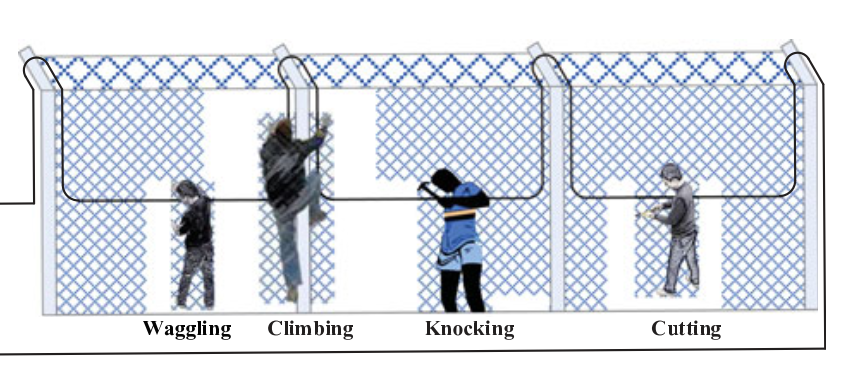
\includegraphics[width=0.7\linewidth]{images/Bab_2/Bab_2_1}
		\caption[Ragam Intrusi]{\small{Sebagian ragam bentuk tindak intrusi}}
	\end{figure}

	\subsection{Serat Optik}
	
	Serat optik merupakan pemandu gelombang silindris dielektrik yang terbuat dari material low-loss seperti plastik maupun gelas silika.
	Serat optik terdiri dari core dimana cahaya dipandu, dan cladding sebagai sebagai selubung core.
	Core memiliki indeks bias lebih tinggi daripada cladding.
	
	\begin{figure}[h!]
		\centering
		\captionsetup{justification=centering}
		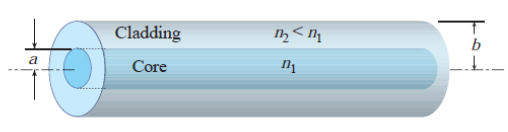
\includegraphics[width=0.7\linewidth]{images/Bab_2/Bab_2_2}
		\caption[Struktur Serat]{\small{Struktur umum serat optik}}
	\end{figure}
	
	Sinar yang masuk pada boundary core-cladding dengan sudut yang lebih besar daripada sudut kritis akan mengalami peristiwa total internal reflection dan akan dipandu melalui core tanpa mengalami pembiasan.
	Berdasarkan moda perambatannaya, serat optik dibagi menjadi dua jenis yaitu serat singlemode yang memiliki diameter core lebih kecil dan serat multimode yang memiliki diameter core lebih besar. 
	Tipe perambatan sinar pada core serat optik dibagi dua yaitu step-index dan graded-index.
	
	\begin{figure}[h!]
		\centering
		\captionsetup{justification=centering}
		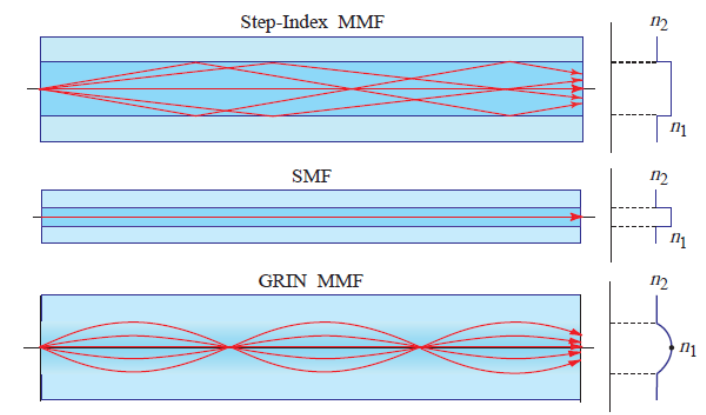
\includegraphics[width=0.7\linewidth]{images/Bab_2/Bab_2_3}
		\caption[Muka Gelombang Serat Optik]{\small{Bentuk Geometri, Profil Indeks Bias dan Tipe Perambatan sinar pada MMF Step, SMF,dan MMF Graded}}
	\end{figure}


	\subsection{Multimode Interference (MMI)}
	
	Multimode Interference (MMI) merupakan fenomena yang terjadi akibat adanya pemantulan cahaya secara berulang didalam susunan core dan cladding pandu gelombang.
	Pemantulan yang berulang didalam core menyebabkan terjadinya interferensi internal, sehingga terjadi perubahan pola cahaya yang keluar dari core secara periodik. 
	Interferensi yang terjadi dapat secara konstruktif maupun destruktif bergantung pada profil indeks bias, jejari, radius, dan panjang gelombang operasi yang digunakan.
	Interferensi konstruktif yang terjadi secara periodik ini disebut sebagai self imaging.
	Fenomena self imaging didalam pandu gelombang multimode dapat dijelaskan menggunakan modal propagation analysis (MPA).
	
	\begin{figure}[h!]
		\centering
		\captionsetup{justification=centering}
		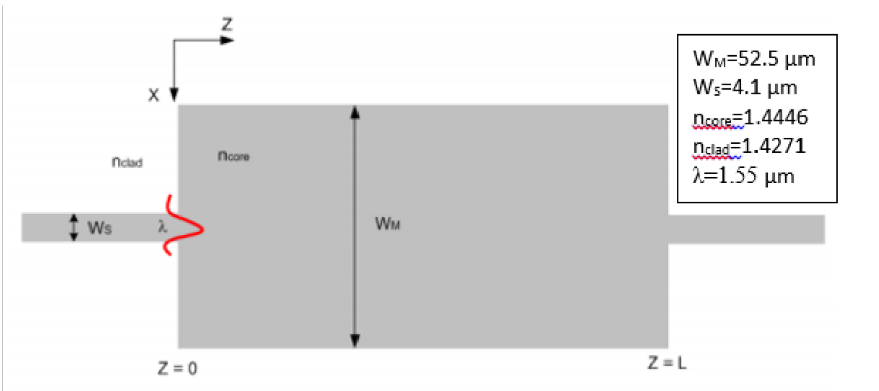
\includegraphics[width=0.7\linewidth]{images/Bab_2/Bab_2_4}
		\caption[Pandu Gelombang SMS]{\small{Skema pandu gelombang multimode pada serat optik SMS}}
	\end{figure}

	Pada profil medan input (z = 0), moda yang berasal dari serat singlemode tereksitasi menjadi distribusi moda yang mungkin terpandu kedalam pandu gelombang serat multimode.
	Sedangkan pada profil medan (z=L), akan menghasilkan self imaging sebanyak n kali dengan jarak tertentu secara periodik (jarak reimaging) .
	Jarak self imaging ditentukan oleh konstanta propagasi antar moda yang berdekatan ($\beta_{m}$ dan $\beta_{m+1}$), dinyatakan sebagai berikut:
	
	\begin{align}
		L_{i} = 10 * \frac{\pi}{\beta_{m} + \beta_{m+1}}
	\end{align}
	
	\subsection{Efek Mekanis pada Serat Optik} 
	
	Efek mekanis disini adalah perlakuan mekanis terhadap serat yang dapat mempengaruhi daya yang dirambatkan oleh serat optik.
	Perlakuan yang dipilih disini adalah macro-bending dimana telah dilakukan penelitian bahwa macro-bending dapat mempengaruhi hasil trace OTDR \cite{Maharinda}.
	
	\subsection{Serat Optik sebagai Distributed Sensor}
	
	Selain sebagai perambat gelombang cahaya, serat optik saat ini juga digunakan sebagai sensor.
	Salah pencapaian dalam serat optik sebagai sensor adalah penggunaannya sebagai distributed sensor \cite{Dakin1992}.
	Pengertian distributed  disini adalah bahwa sepanjang serat optik dapat berfungsi sebagai sensor dan menggantikan model sensor konvensional yang berbasis pengukuran satu titik \cite{Wu2015}.
	Penggunaan distributed sensor ini tentu akan mengurangi biaya dan kompleksitas sistem.
	
	\subsection{Optical Time Domain Reflectometer (OTDR)}
	
	OTDR atau Optical Time Domain Reflectometer adalah alat untuk karakterisasi serat optik yang bekerja dengan mentransmisikan berkas laser dalam bentuk pulsa kemudian mengukur sinyal balik di setiap cacah waktu \cite{test2017}.
	Sinyal balik dalam OTDR merupakan hasil dari fenomena backscattering.
	Skema OTDR secara umum adalah sebagai berikut:
	
	\begin{figure}[h!]
		\centering
		\captionsetup{justification=centering}
		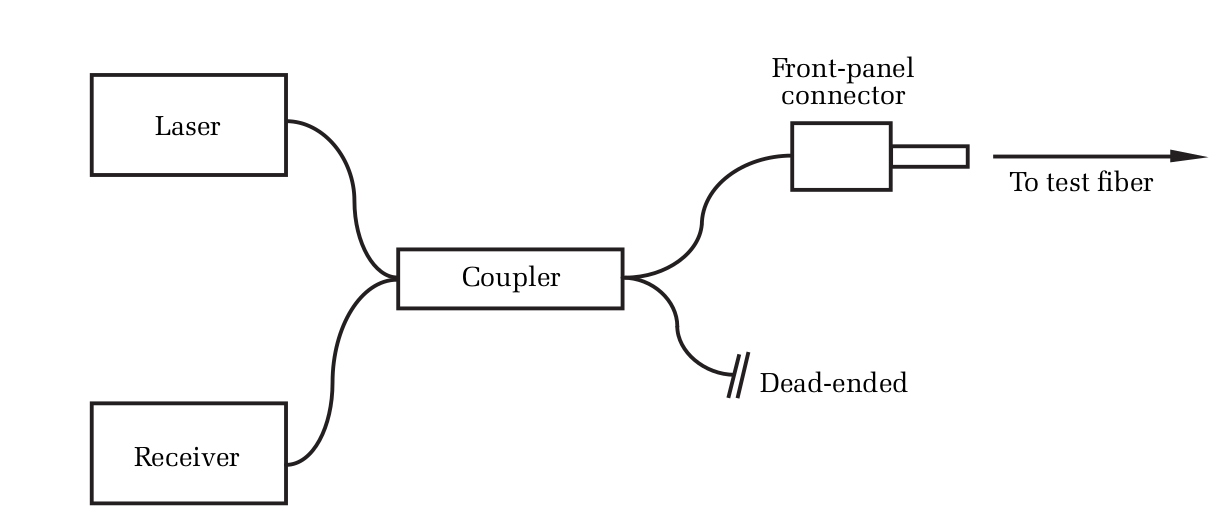
\includegraphics[width=0.65\linewidth]{images/Bab_2/Bab_2_5}
		\caption[Struktur umum OTDR]{\small{Struktur umum OTDR}}
	\end{figure}

	Hasil pengukuran OTDR atau yang sering disebut trace adalah berupa plot nilai pelemahan daya backscatter terhadap waktu atau panjang serat optik \cite{Anderson2004}.
	Berikut adalah tipikal plot trace dalam OTDR:
	
	\begin{figure}[h!]
		\centering
		\captionsetup{justification=centering}
		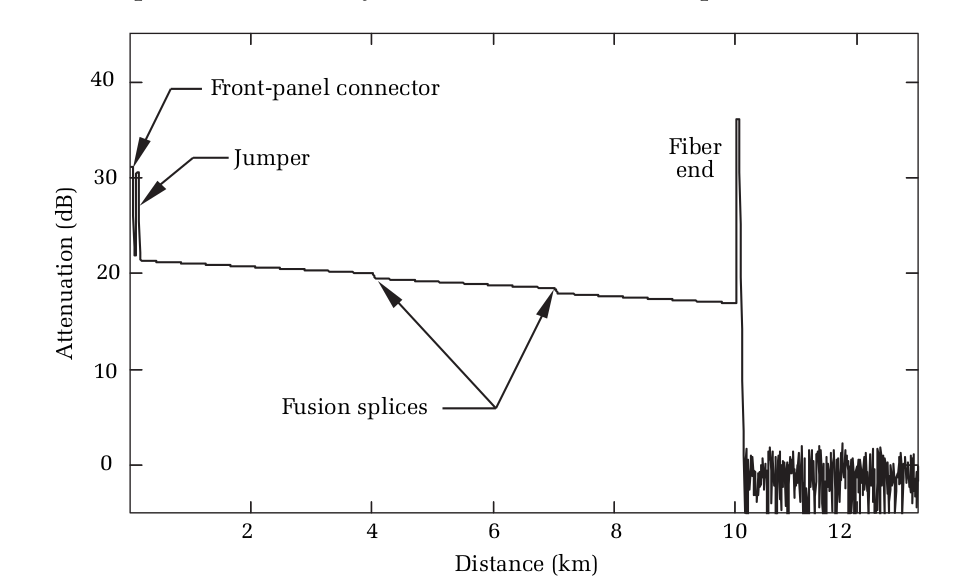
\includegraphics[width=0.7\linewidth]{images/Bab_2/Bab_2_6}
		\caption[Tipikal plot hasil OTDR]{\small{Tipikal plot hasil OTDR}}
	\end{figure}

	Di dalam hasil hasil trace akan menunjukkan respon terhadap events baik berupa reflective maupun non-reflective.
	
	\begin{figure}[h!]
		\centering
		\captionsetup{justification=centering}
		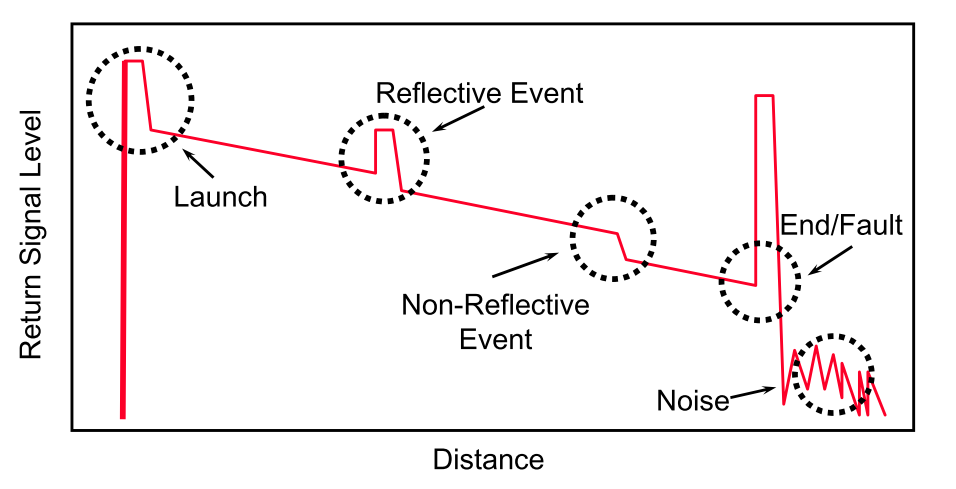
\includegraphics[width=0.7\linewidth]{images/Bab_2/Bab_2_7}
		\caption[respon events hasil OTDR]{\small{respon events hasil OTDR \cite{Anritsu2010}}}
	\end{figure}

	\subsection{Backscattering}
	
	Fenomena backscattering merupakan fenomena yang diakibatkan oleh respon material silikat dari serat optik terhadap pulsa laser yang ditransmisikan oleh OTDR.
	Scattering yang terjadi dapat berupa Raleigh (RB) maupun stimulated Brillouin (SBS) \cite{Feng2017}.
	Berikut adalah skema umum dari backscattering:
	
	\begin{figure}[h!]
		\centering
		\captionsetup{justification=centering}
		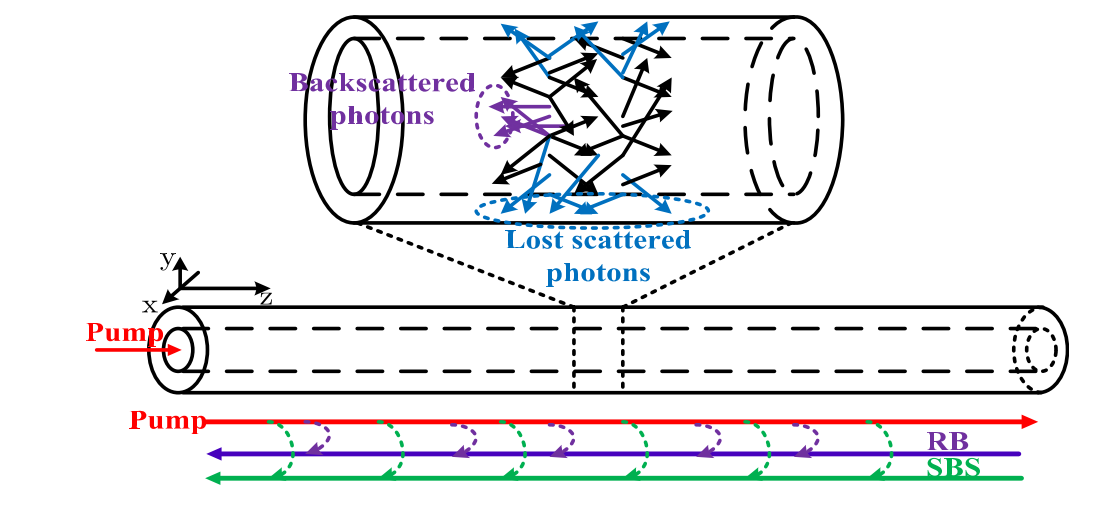
\includegraphics[width=0.4\linewidth]{images/Bab_2/Bab_2_8}
		\caption[Skema umum backscatter.]{\small{Skema umum backscatter.}}
	\end{figure}

	\subsection{Modul OTDR Anritsu MU909015C}
	
%=============================================================================

\newpage
\thispagestyle{plain}
\mbox{}

%=============================================================================
% BAB III 

\newpage

	\setcounter{figure}{0}

	\section{Metodologi}
	
	\begin{center}
		{\large \textbf{BAB III}} \\
		{\large \textbf{Metodologi}}
	\end{center}
	
	\subsection{Tempat  Penelitian}
	
	Penelitian ini akan dilakukan di Laboratorium Rekayasa Fotonika dan lingkungan sekitar gedung Jurusan Teknik Fisika ITS.
	
	\subsection{Prosedur Penelitian}
	
	Prosedur penelitian terdiri dari beberapa tahapan yang dilakukan dari awal hingga akhir untuk tercapainya tujuan dari penelitian ini.
	Metode penelitian merupakan serangkaian kegiatan yang dilakukan dari awal higga akhir untuk tercapainya tujuan penelitian ini.
	
	\begin{figure}[h!]
		\centering
		\captionsetup{justification=centering}
		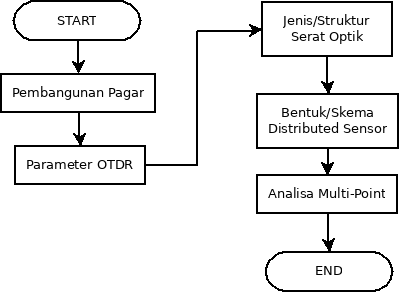
\includegraphics[width=0.5\linewidth]{images/Bab_3/Bab_3_1}
		\caption[Diagram Alir Penelitian]{\small{Diagram Alir Penelitian}}
	\end{figure}

	Prosedur penelitian dibagi menjadi beberapa tahapan yang akan dijelaskan rinci sebagai berikut :
	
	\subsection{Pembuatan Pagar}
	
	Untuk dapat dilakukan penelitian tentang deteksi intrusi, maka direncanakan pembangunan pagar tipe harmonika di belakang gedung E sepanjang 10 m dan setinggi 1 m berbahan kawat dengan rangka berbahan baja seamless tubular.
	Skema akhir seluruhnya mencakup pagar, OTDR, serat optik, gulungan, dan komputer.
	Distributed sensor divariasikan pada puncak pagar dan setiap jarak 25 cm pada tinggi harmonika pagar untuk dapat mendeteksi setiap kemungkunan tindak penyusupan \cite{Huang2017}.
	Berikut adalah gambaran setup yang akan dibangun ditunjukkan pada Gambar 3.2.
	
	\begin{figure}[h!]
		\centering
		\captionsetup{justification=centering}
		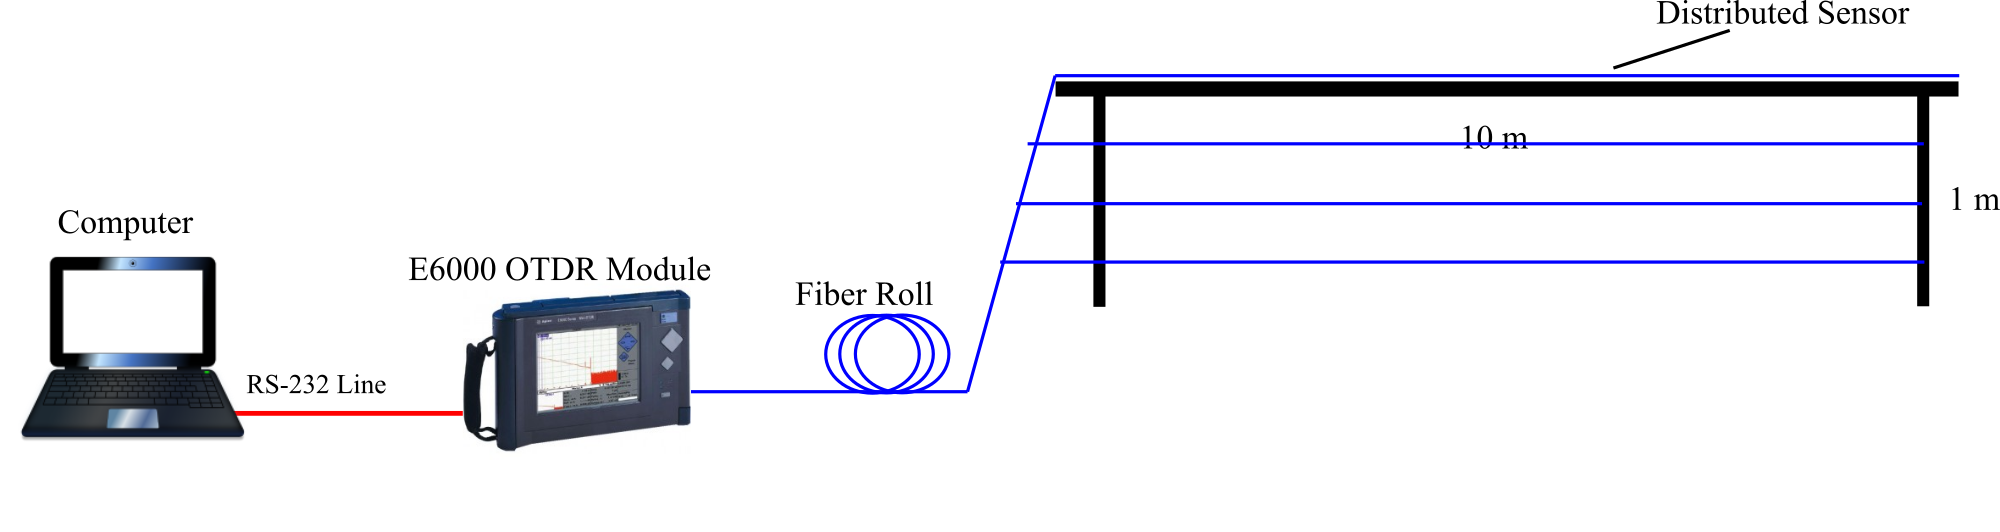
\includegraphics[width=0.5\linewidth]{images/Bab_3/Bab_3_2}
		\caption[Skema Setup]{\small{Skema setup secara global}}
	\end{figure}

	Tahap selanjutnya adalah penentuan nilai parameter OTDR yang dapat menghasilkan hasil trace dengan events yang distinguishable. Parameter yang dimaksud adalah nilai lebar pulsa (Pulse-Width) dan periode pulsa.
	Berikut gambar 3.3 diagram alir tahap ini:
	
	\begin{figure}[h!]
		\centering
		\captionsetup{justification=centering}
		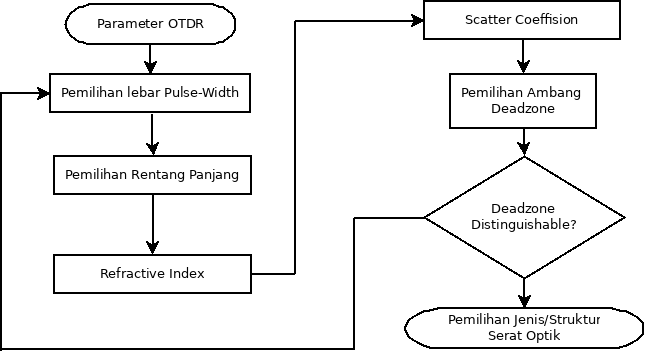
\includegraphics[width=0.5\linewidth]{images/Bab_3/Bab_3_3}
		\caption[Parameter OTDR ]{\small{Diagram Alir Penentuan Parameter OTDR }}
	\end{figure}

	Penentuan nilai-nilai parameter ini dapat dilakukan di module sendiri melalui software antar muka pada module OTDR.
	
	\begin{figure}[h!]
		\centering
		\captionsetup{justification=centering}
		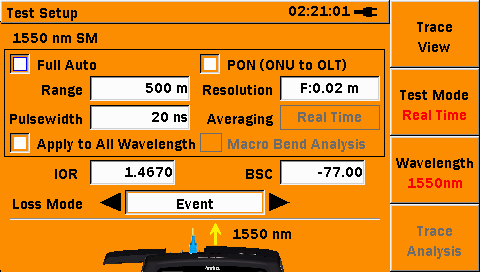
\includegraphics[width=0.5\linewidth]{images/Bab_3/Bab_3_4}
		\caption[panel antar-muka module]{\small{Panel antar-muka module }}
	\end{figure}

	\begin{figure}[h!]
		\centering
		\captionsetup{justification=centering}
		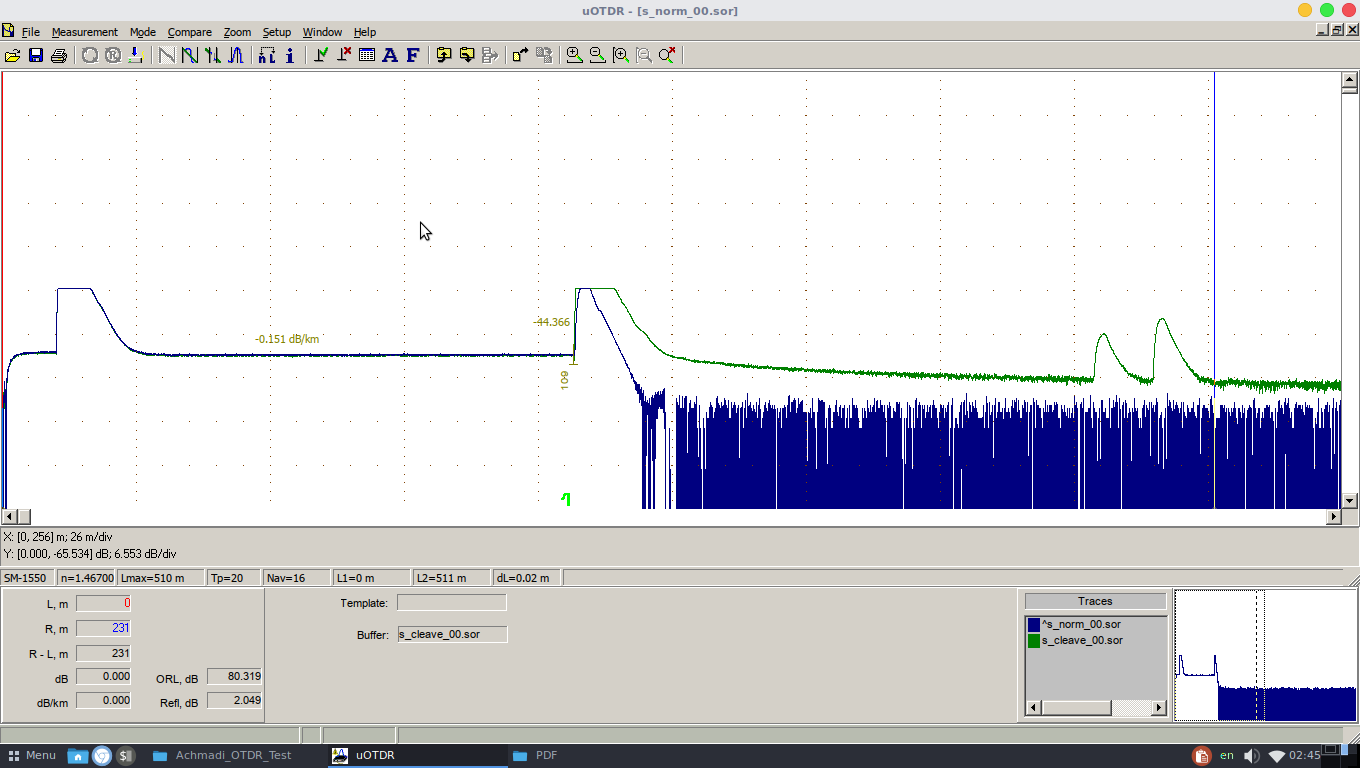
\includegraphics[width=0.7\linewidth]{images/Bab_3/Bab_3_5}
		\caption[Trace Viewer pada Komputer]{\small{Trace Viewer pada Komputer}}
	\end{figure}

	\subsection{Jenis/Struktur Serat Optik}
	
	Tahapan ini bertujuan untuk membandingkan penggunaan jenis dan struktur yang berbeda dari serat optik untuk mendapatkan hasil trace dengan events yang paling distinguishable.
	Variasi jenis serat optik adalah \cite{Hafid2014}:
	
	\begin{itemize}
		\item Single-Mode (step-index)
		\item Multi-Mode (graded-index)
	\end{itemize}

	Sedangkan variasi struktur adalah 1) single-structure dan 2) multi-structure berstruktur Single-Multi-Single \cite{Diana}.
	Berikut diagram alir tahapan ini:
	
	\begin{figure}[h!]
		\centering
		\captionsetup{justification=centering}
		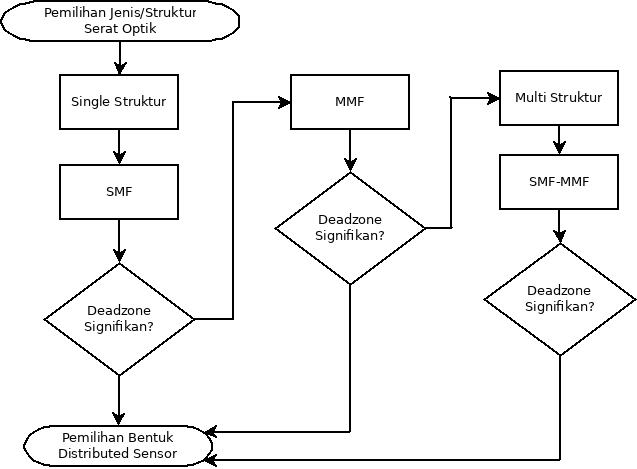
\includegraphics[width=0.8\linewidth]{images/Bab_3/Bab_3_6}
		\caption[Diagram Alir]{\small{Diagram Alir pemilihan jenis/struktur serat optik}}
	\end{figure}
	
%	\subsection{Bentuk/Skema Distributed Sensor}
%	
%	Tahapan ini bertujuan untuk membandingkan setup distributed sensor  yang nantinya akan diimplimentasikan pada pagar.
%	Variasi bentuk/skema adalah:
%	
%	\begin{itemize}
%		\item tanpa bentuk tertentuk
%		\item bentuk lilitan
%		\item bentuk S
%		\item bentuk 8
%	\end{itemize}
%
%	Selain variasi bentuk/skema, juga dilakukan variasi jumlah di setiap bentuk/skema.
%	Setelah semua dilakukan pengujian maka distributed sensor diimplementasikan ke struktur pagar. 
%	Berikut diagram alir tahapan ini:
%	
%	\begin{figure}[h!]
%		\centering
%		\captionsetup{justification=centering}
%		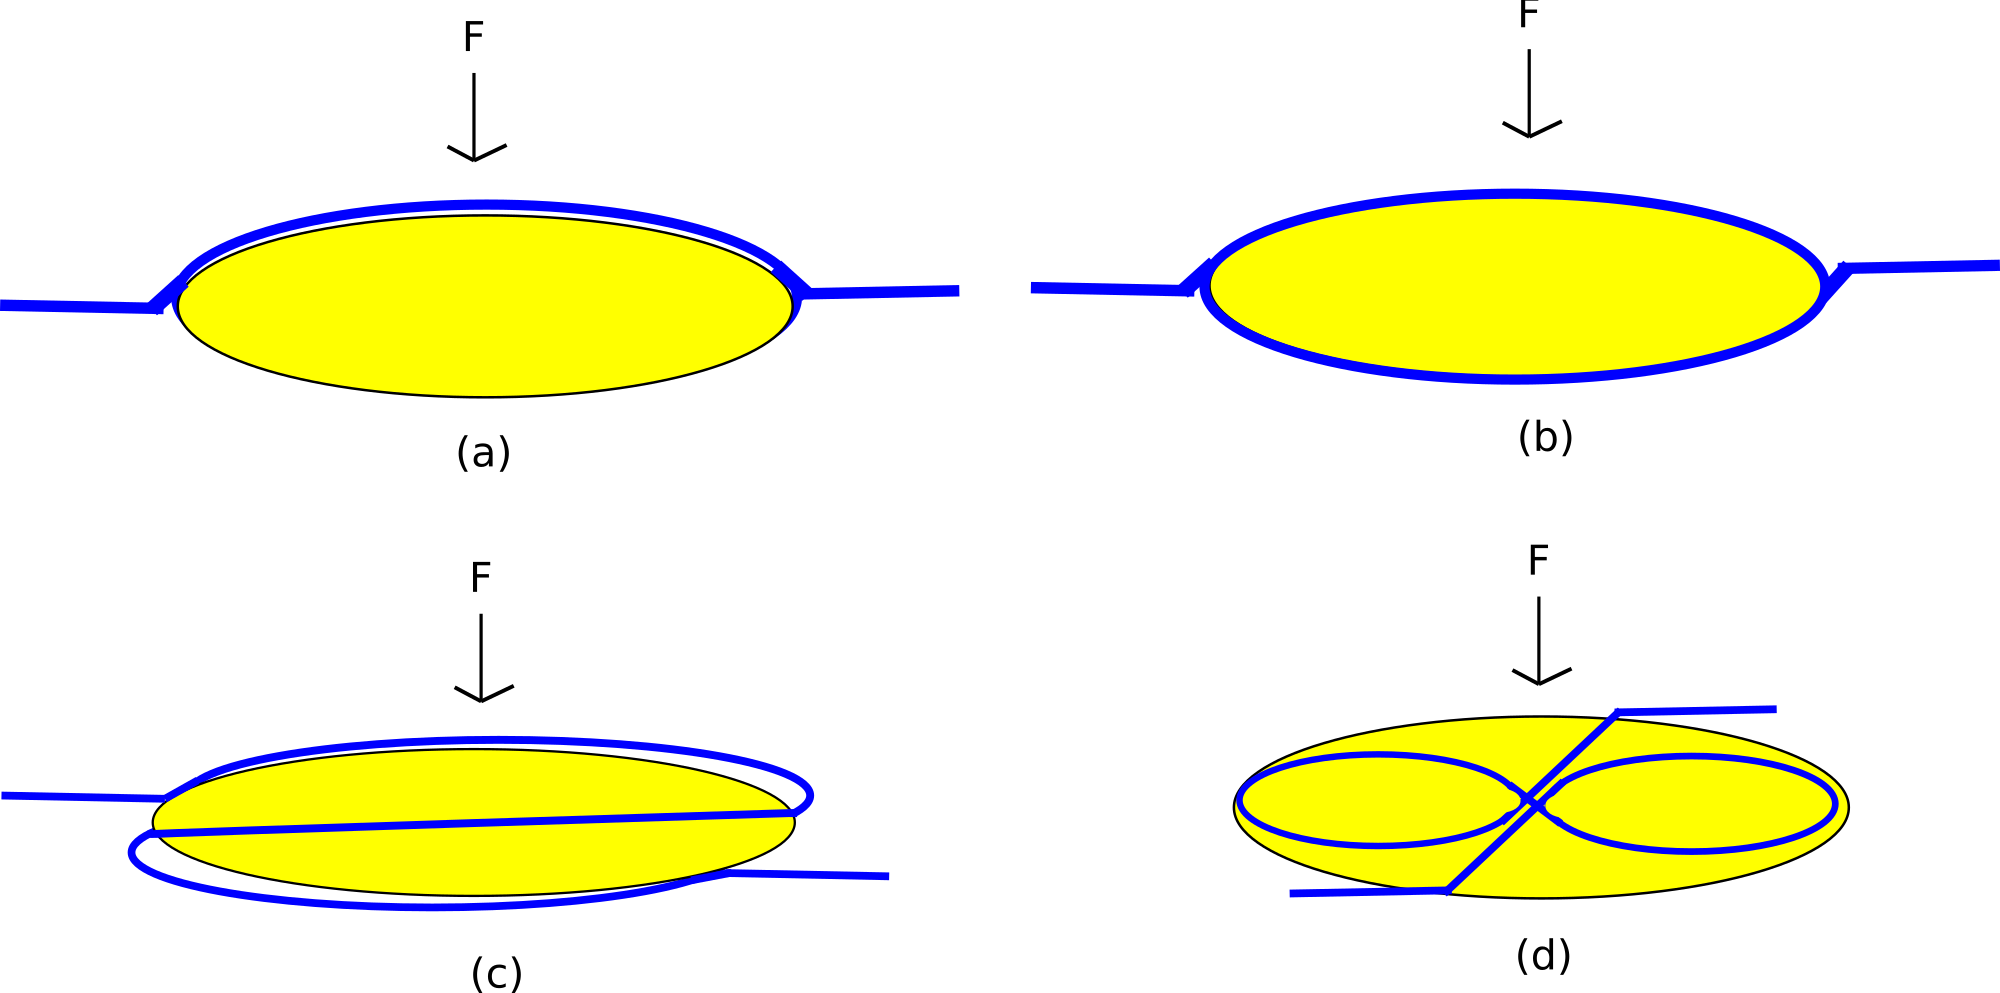
\includegraphics[width=0.7\linewidth]{images/Bab_3/Bab_3_7}
%		\caption[Skema Uji]{\small{(a) Tanpa bentukan tertentu, (b) lilitan, (c) bentuk S, dan (d) bentuk 8}}
%	\end{figure}
%
%	Warna kuning dalam skema di atas adalah bantalan yang berfungsi sebagai 1) peredam gaya tekan dan 2) memberi bentuk default kepada distributed sensor.
%	Nilai F sebagai pembebanan diambil sebesar massa rata-rata pria dewasa yaitu 70 kg \cite{Huang2017}.
%	Sedangkan jumlahnya maka mengacu bahwa ukuran lebar manusia berkisar antara 70 cm hingga 120 cm \cite{Ramsey1980}, maka diambil 100 cm sebagai standar sehingga jumlah maksimal adalah 10 titik.
%	
%=============================================================================
\newpage
	\subsection{Analisa Multi-Point}
	
	Tahapan terakhir dalam penelitian ini adalah tahap analisa hasil trace untuk menentukan jumlah gangguan multi-point pada pagar secara akurat.
	Analisa dilakukan dengan mengambil hasil trace sebagai sinyal periodik domain waktu untuk mendapatkan jumlah titik dengan amplitudo yang tergolong events.
	Hasil analisa ini kemudian digeneralisasi sehingga dapat dituangkan ke dalam bentuk algoritma yang dapat digunakan untuk menghitung jumlah gangguan secara real-time.
	Berikut diagram alir tahapan ini:
	
	\begin{figure}[h!]
		\centering
		\captionsetup{justification=centering}
		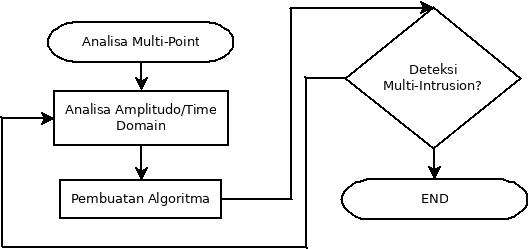
\includegraphics[width=0.8\linewidth]{images/Bab_3/Bab_3_8}
		\caption[Diagram Alir]{\small{Diagram Alir analisa multi-point dari hasil trace}}
	\end{figure}
	
%=============================================================================
% BAB IV
\newpage

	\setcounter{figure}{0}
	
	\section{Hasil}
	
	\begin{center}
		{\large \textbf{BAB IV}} \\
		{\large \textbf{Hasil dan Pembahasan}}
	\end{center}

	Berikut adalah hasil eksperimen awal untuk menguji respon OTDR dari serat optik dalam kondisi yang telah ditentukan kemudian diberi peturbation (gangguan) berupa macro-bending di satu tempat.
	
	\subsection{Gangguan}
	
	Gangguan yang digunakan untuk eksperimen awal disini berupa macro-bending yang berasal dari dua perlakuan, yaitu tekanan yang dikenakan pada busa elastis yang telah dililitkan serat optik dan tekanan yang dikenakan pada pelat besi lunak.
	
	
	\begin{enumerate}
		\item Berikut adalah gambaran busa elastis sebagai alat bantu untuk membentuk bending pada serat optik.
	
			\begin{figure}[h!]
				\centering
				\captionsetup{justification=centering}
				\begin{subfigure}[b]{0.3\textwidth}
					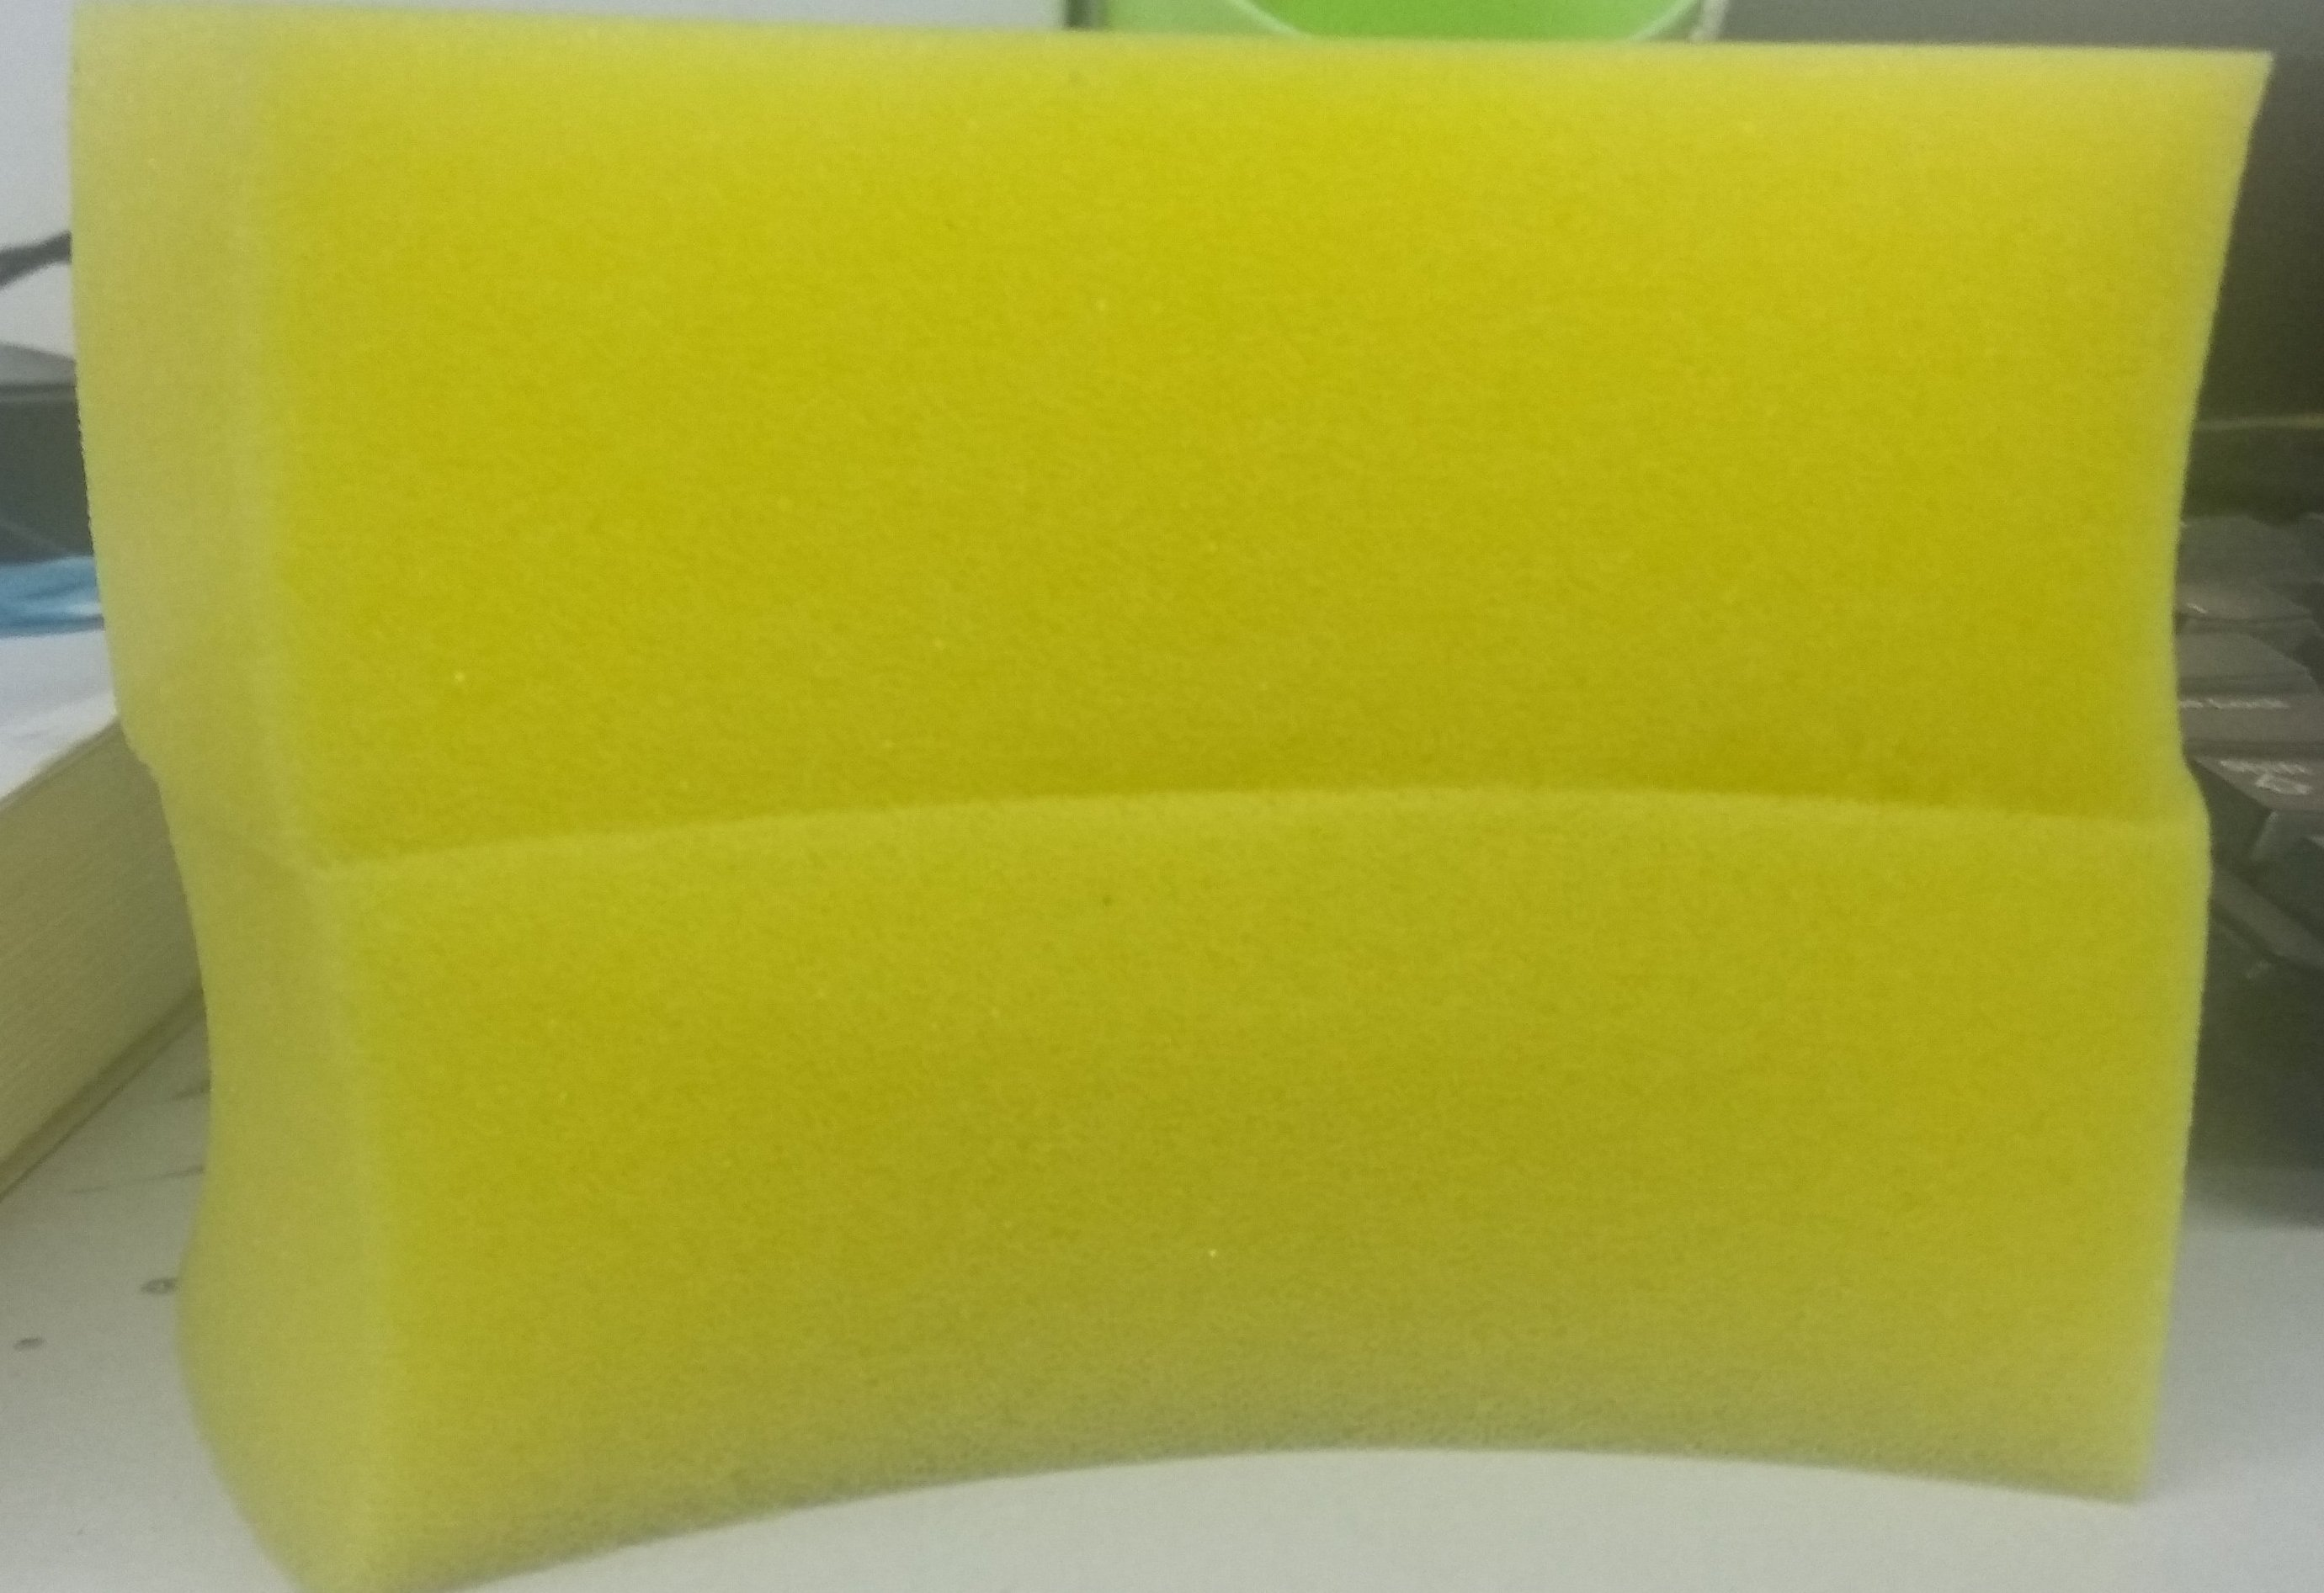
\includegraphics[width=\textwidth]{images/Bab_4/Bab_4_1a}	
					\caption{\small{kondisi normal asli}}		
				\end{subfigure}
				\begin{subfigure}[b]{0.3\textwidth}
					
\includegraphics[width=\linewidth]{images/Bab_4/Bab_4_1b}
					\caption{\small{diagram normal}}			
				\end{subfigure}
				\begin{subfigure}[b]{0.3\textwidth}
					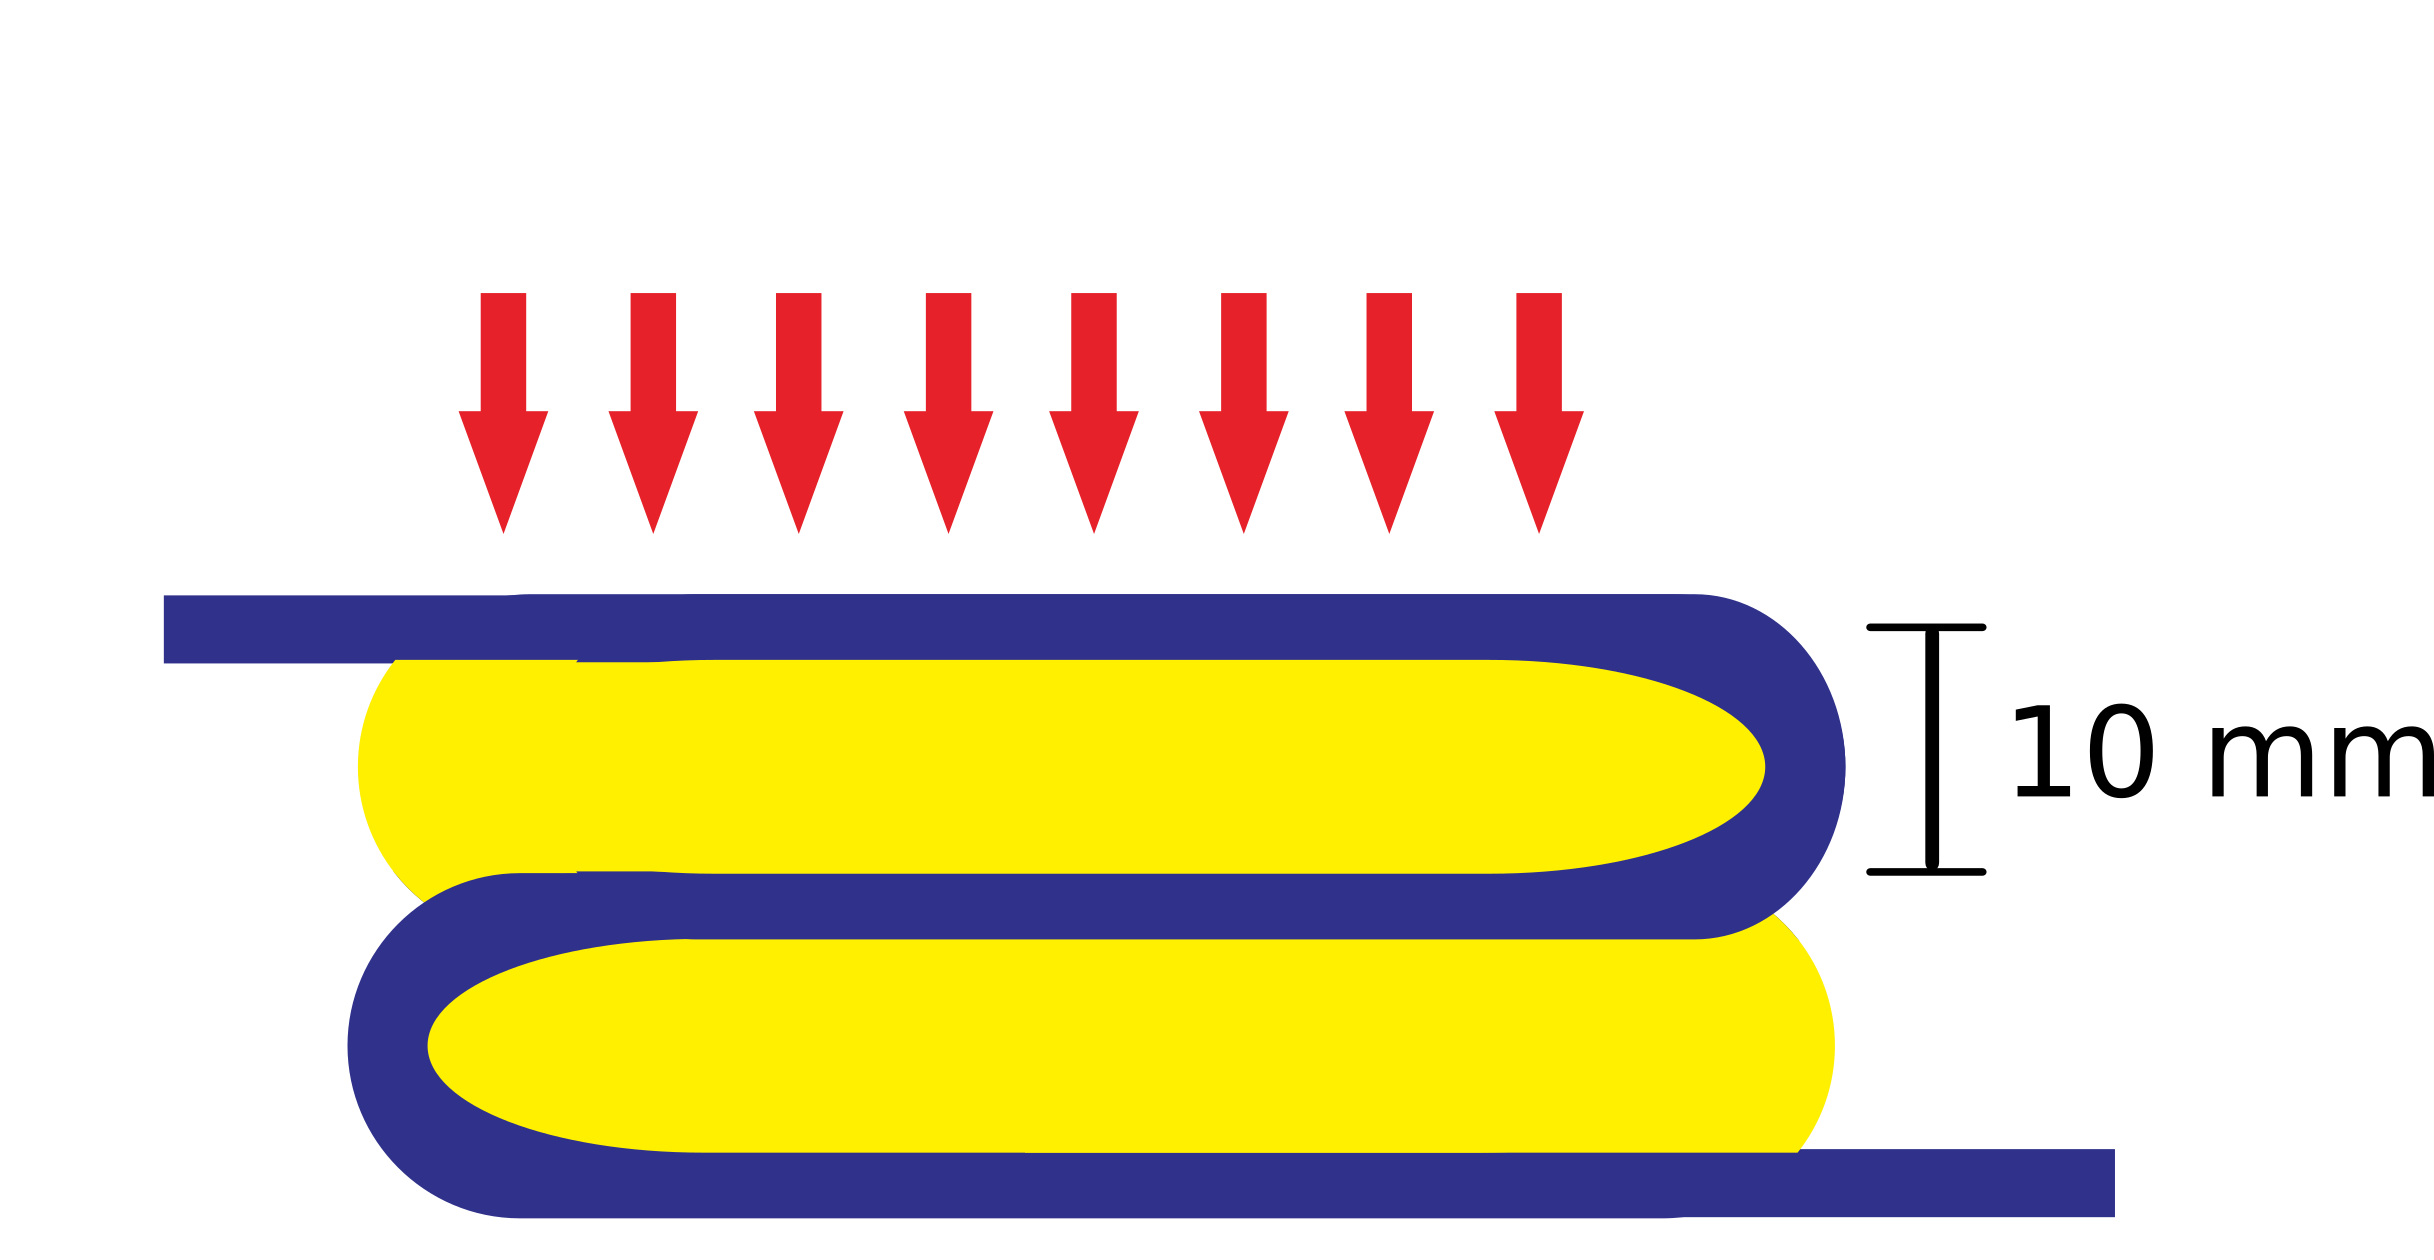
\includegraphics[width=\linewidth]{images/Bab_4/Bab_4_1c}
					\caption{\small{diagram dikenakan tekanan}}			
				\end{subfigure}
				\caption[Uji Peturbasi]{\small{Gambaran gangguan terhadap serat optik}}
			\end{figure}
		
		\item Berikut adalah gambaran pelat besi lunak sebagai alat bantu untuk membentuk bending pada serat optik.
		
			\begin{figure}[h!]
				\centering
				\captionsetup{justification=centering}
				\begin{subfigure}[b]{0.2\textwidth}
					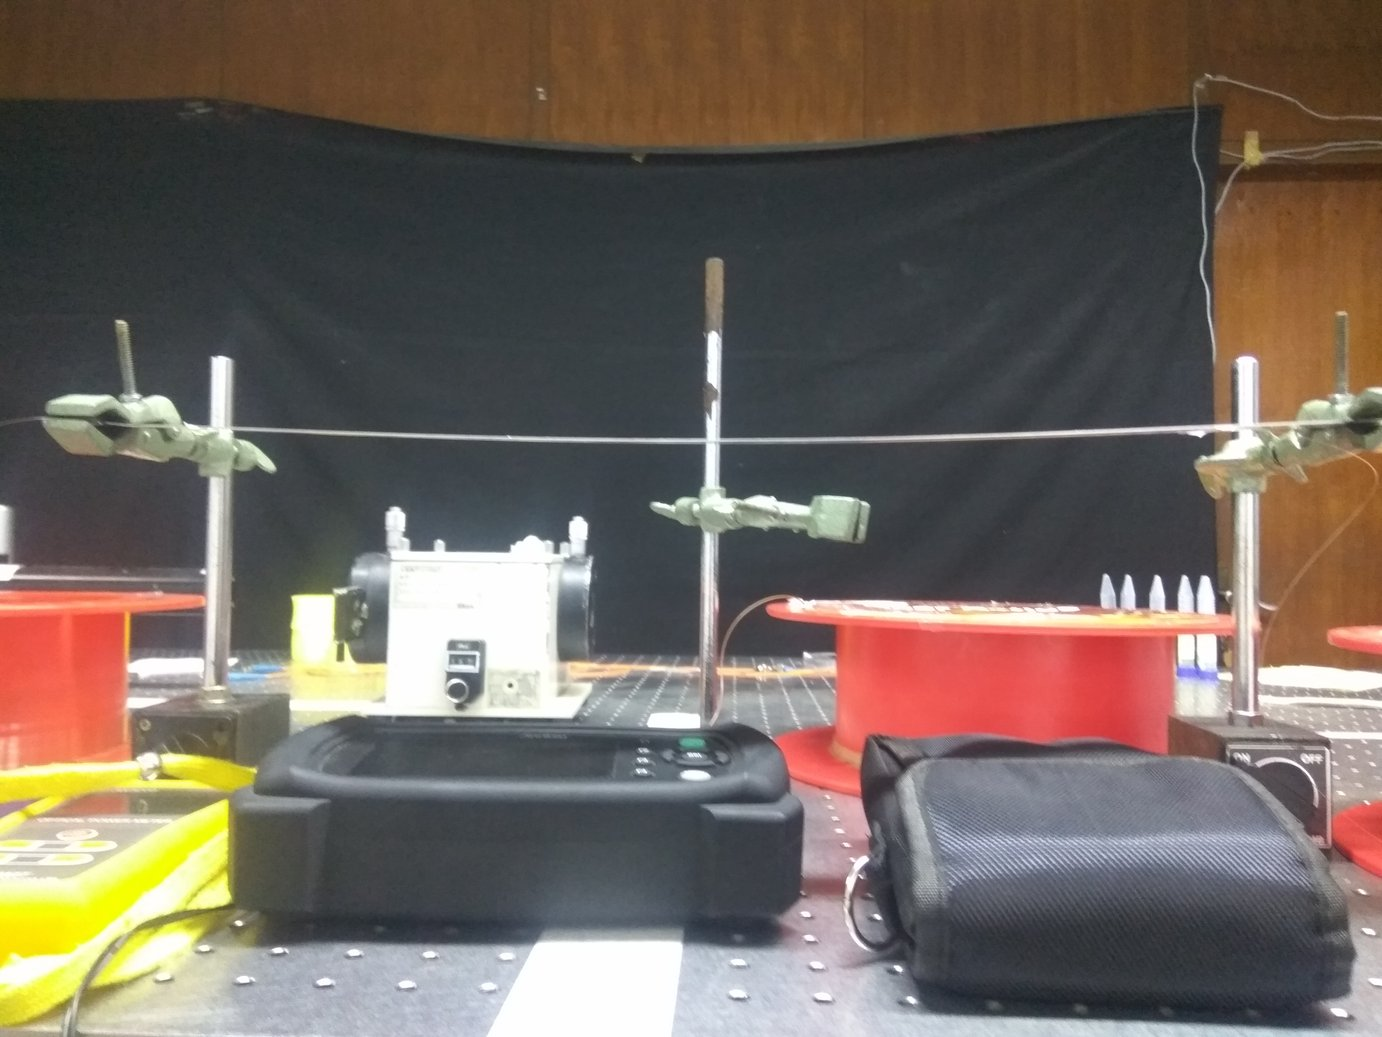
\includegraphics[width=\textwidth]{images/Bab_4/Bab_4_2a}	
					\caption{\small{kondisi normal asli}}		
				\end{subfigure}
				\begin{subfigure}[b]{0.2\textwidth}
					
\includegraphics[width=\linewidth]{images/Bab_4/Bab_4_2b}
					\caption{\small{diagram bending pelat}}			
				\end{subfigure}
				\caption[Uji Peturbasi]{\small{Gambaran gangguan terhadap serat optik }}
			\end{figure}
		
	\end{enumerate}

	\subsection{Parameter sementara OTDR}
	
	Dalam eksperimen ini digunakan parameter OTDR dari eksperimen serat opti SMS sebagai sensor arus \cite{Hafid2014},
	yaitu nilai Index of Reflection (IOR) sebesar 1.4670 dan BackScatter Coefficient (BSC) senilai -77.
	Sedangkan untuk panjang gelombang digunakan 1550 nm. 
	
	\subsection{Hasil uji di setiap perlakukan }
	
	Berikut dipaparkan hasil setiap perlakuan disertai pembandingan, sehingga dapat diketahui perbedaan respon OTDR di setiap perlakuan.
	
	\begin{enumerate}
		\item \textbf{Single Mode}

		Berikut adalah hasil trace OTDR untuk serat optik SMF dengan satu splice yaitu antara 1 roll SMF 100m dengan 10 cm SMF dengan konektor FC (pigtailed)
		
		\begin{figure}[h!]
			\centering
			\captionsetup{justification=centering}
			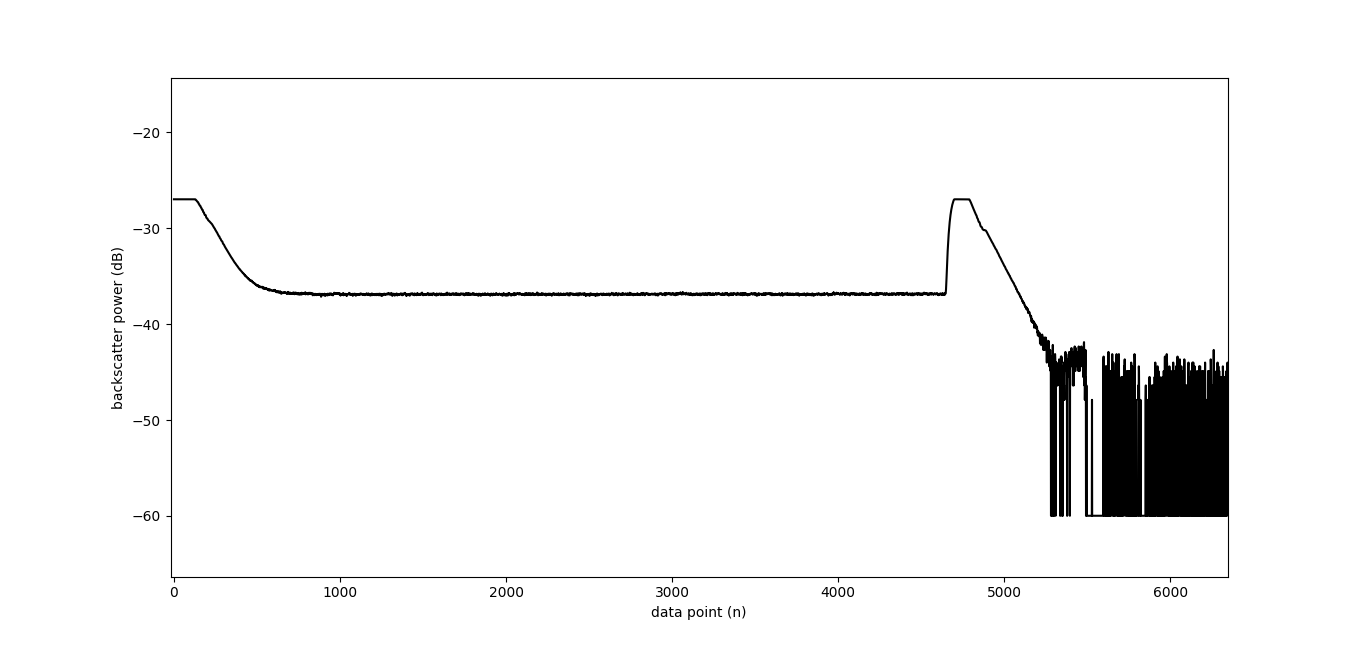
\includegraphics[width=0.5\linewidth]{images/Bab_4/Bab_4_3a1}
			\caption[Trace SMF]{\small{Hasil trace OTDR pada SMF normal}}
		\end{figure}
		
		\item \textbf{Single Mode – Single Mode}
		
		Berikut adalah hasil trace OTDR untuk serat optik SMF dengan dua splice yaitu antara 1 roll SMF 100m, 1 roll SMF 50m, dan 10 cm SMF dengan konektor FC (pigtailed).
		
		\begin{figure}[h!]
			\centering
			\captionsetup{justification=centering}
			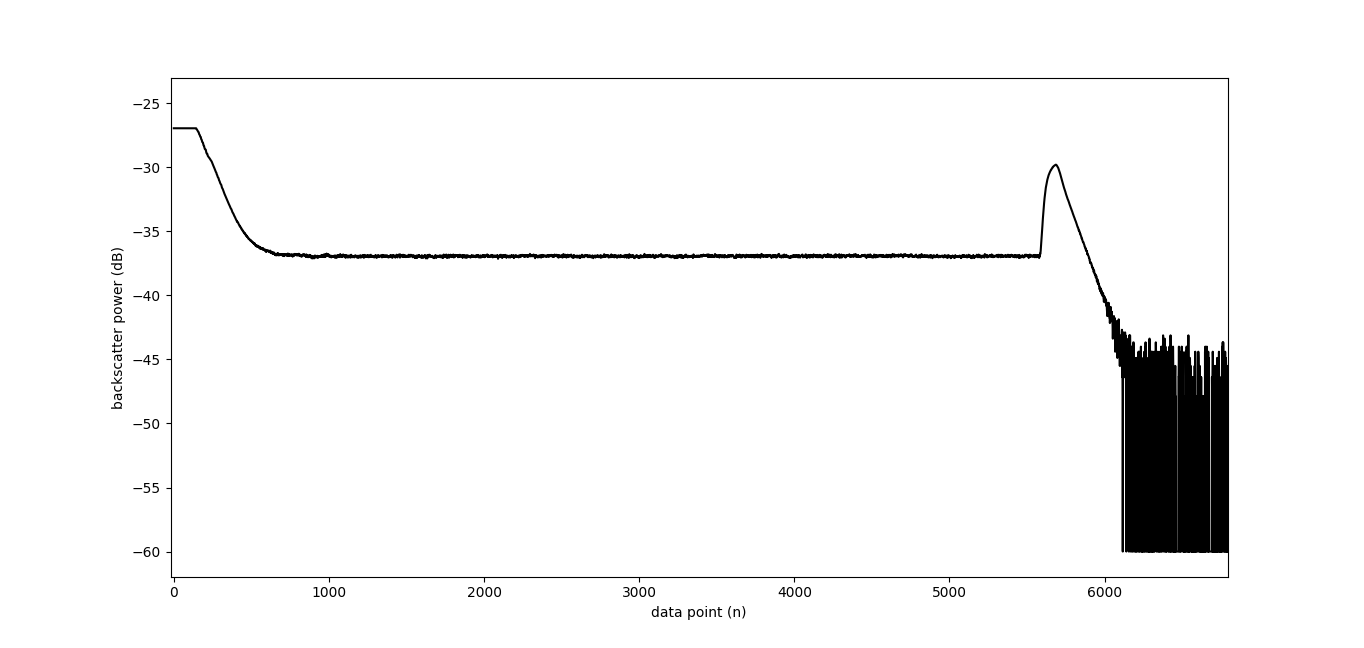
\includegraphics[width=0.5\linewidth]{images/Bab_4/Bab_4_3b1}
			\caption[Trace SMF-SMF]{\small{Hasil trace OTDR pada SM-SM normal}}
		\end{figure}
		
		\begin{figure}[h!]
			\centering
			\captionsetup{justification=centering}
			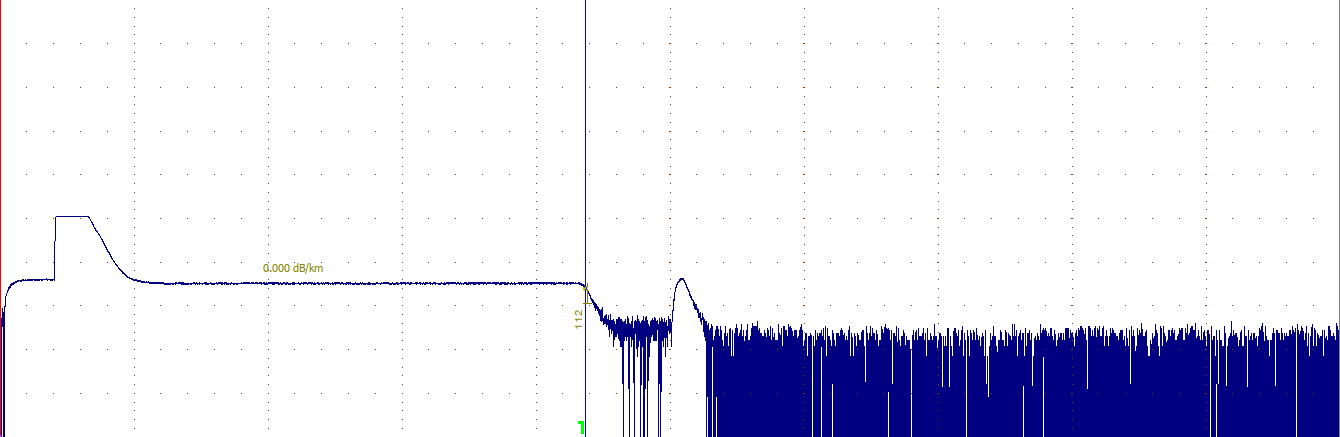
\includegraphics[width=0.5\linewidth]{images/Bab_4/Bab_4_3b2}
			\caption[Trace SMF-SMF]{\small{Hasil trace OTDR pada SM-SM dengan gangguan}}
		\end{figure}
		
%=============================================================================

\newpage	
		
		\item \textbf{Single Mode – Multi Mode Graded Index}
		
		Berikut adalah hasil trace OTDR untuk serat optik SMF dengan dua splice yaitu antara 1 roll SMF 100m, 1 roll MMF-GI 100m, dan 10 cm SMF dengan konektor FC (pigtailed).
		
		\begin{figure}[h!]
			\centering
			\captionsetup{justification=centering}
			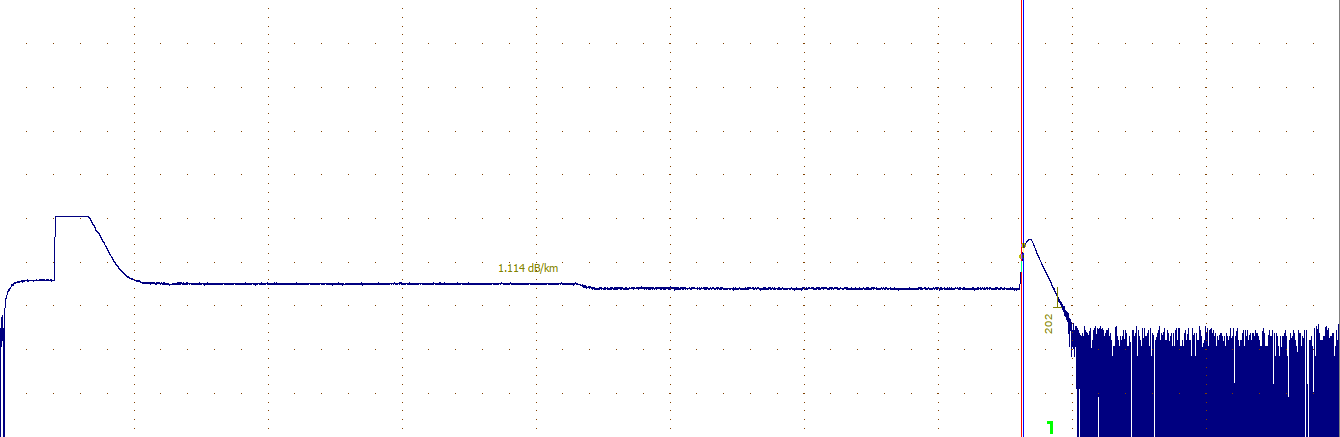
\includegraphics[width=0.5\linewidth]{images/Bab_4/Bab_4_3c1}
			\caption[Trace SM-MMFGI ]{\small{Hasil trace OTDR pada SM-MMFGI normal}}
		\end{figure}
		
		\begin{figure}[h!]
			\centering
			\captionsetup{justification=centering}
			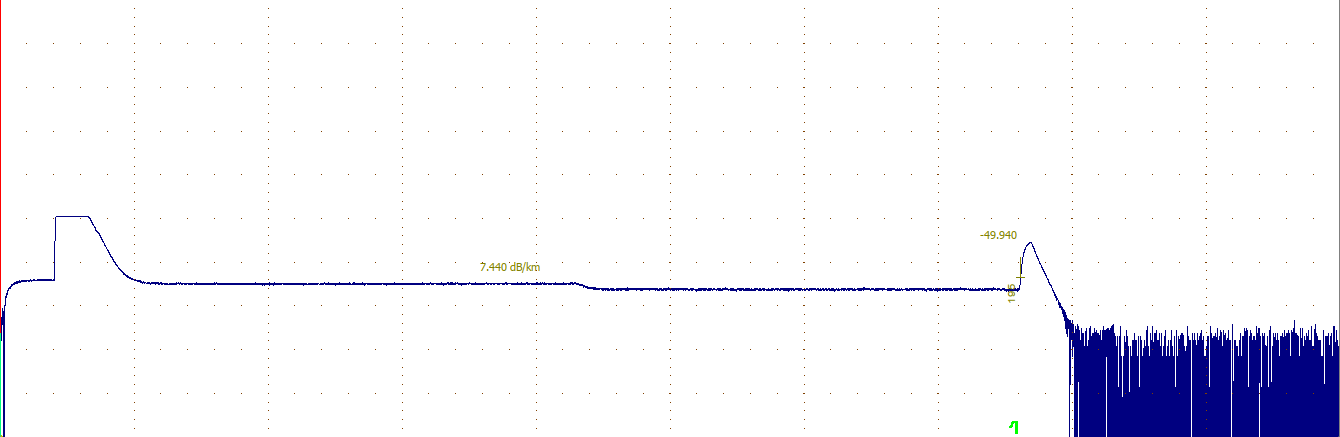
\includegraphics[width=0.5\linewidth]{images/Bab_4/Bab_4_3c2}
			\caption[Trace SM-MMFGI ]{\small{Hasil trace OTDR pada SM-MMFGI dengan gangguan}}
		\end{figure}
		
		\item \textbf{Single Mode – Multi Mode Graded Index - Single Mode }
		
		Berikut adalah hasil trace OTDR untuk serat optik SMF dengan tiga splice yaitu antara 1 roll SMF 100m, 1 roll MMF-GI 100m, 1 roll SMF 20 m, dan 10 cm SMF dengan konektor FC (pigtailed)
		
		\begin{figure}[h!]
			\centering
			\captionsetup{justification=centering}
			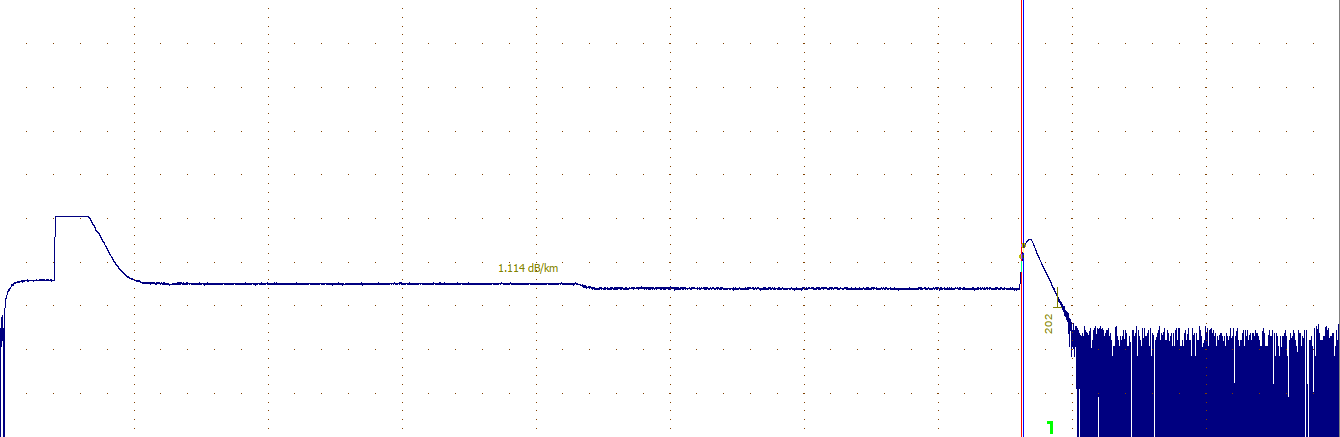
\includegraphics[width=0.5\linewidth]{images/Bab_4/Bab_4_3c1}
			\caption[Trace SM-MMFGI-SM]{\small{Hasil trace OTDR pada SM-MMFGI-SM normal}}
		\end{figure}
		
		\begin{figure}[h!]
			\centering
			\captionsetup{justification=centering}
			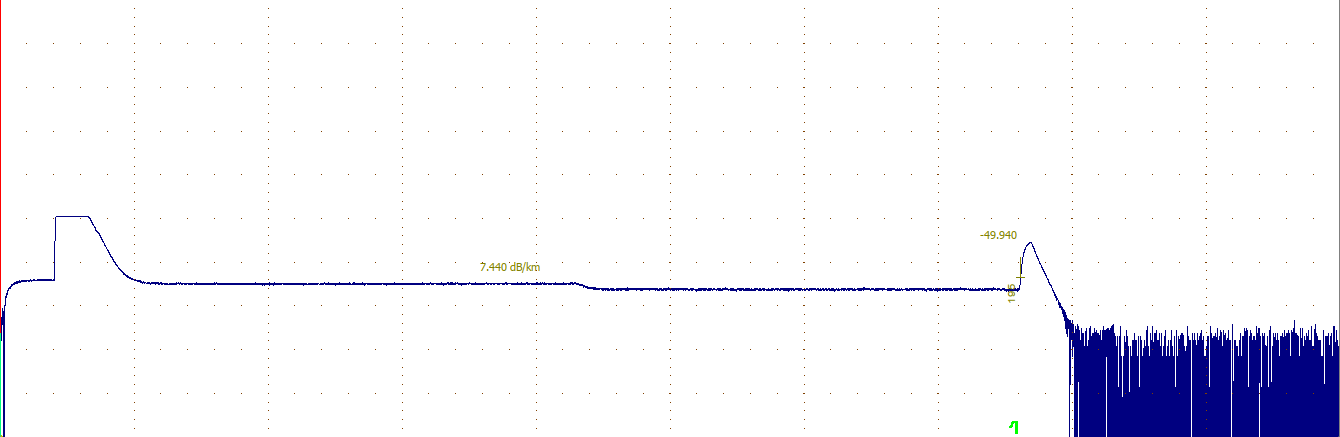
\includegraphics[width=0.5\linewidth]{images/Bab_4/Bab_4_3c2}
			\caption[Trace SM-MMFGI-SM]{\small{Hasil trace OTDR pada SM-MMFGI-SM dengan gangguan}}
		\end{figure}
		
		\item \textbf{Single Mode – Multi Mode Step Index}
		
		Berikut adalah hasil trace OTDR untuk serat optik SMF dengan tiga splice yaitu antara 1 roll SMF 100m, 1 roll MMF-SI 100m, dan 10 cm SMF dengan konektor FC (pigtailed)
		
		\begin{figure}[h!]
			\centering
			\captionsetup{justification=centering}
			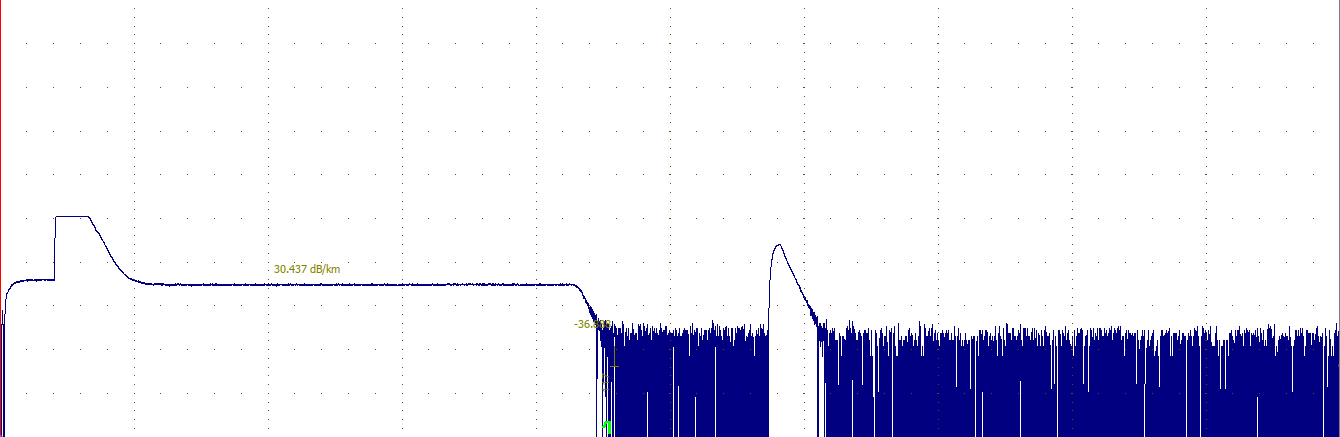
\includegraphics[width=0.5\linewidth]{images/Bab_4/Bab_4_3e1}
			\caption[Trace SM-MMFSI]{\small{Hasil trace OTDR pada baik SM-MMFSI normal maupun SM- MMFSI dengan gangguan}}
		\end{figure}
	
%=============================================================================
\newpage	
	
		\item \textbf{Single Mode – Multi Mode Step Index- Single Mode }
		
		Berikut adalah hasil trace OTDR untuk serat optik SMF dengan tiga splice yaitu antara 1 roll SMF 100m, 1 roll MMF-SI 50m, 1 roll SMF 20 m, dan 10 cm SMF dengan konektor FC (pigtailed).
		
		\begin{figure}[h!]
			\centering
			\captionsetup{justification=centering}
			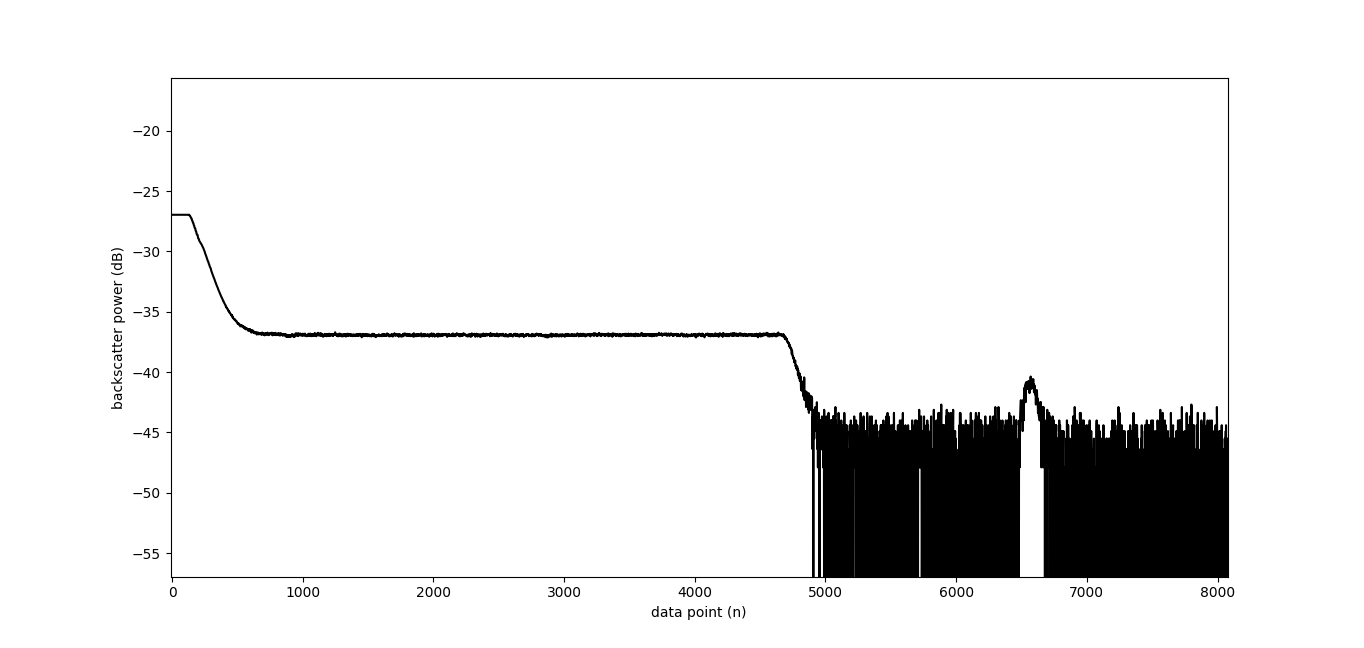
\includegraphics[width=0.5\linewidth]{images/Bab_4/Bab_4_3f1}
			\caption[Trace SM-MMFSI-SM ]{\small{Hasil trace OTDR pada baik SM-MMFSI-SM  normal maupun SM-MMFSI-SM  dengan gangguan}}
		\end{figure}
	
		\item \textbf{Single Mode – Multi Mode Graded dengan pembanding OPM-OLS}
		
		Berikut adalah hasil trace OTDR untuk serat optik SMF dengan tiga splice yaitu antara 1 roll SMF 100m, 1 roll MMF-SI 50m, 1 roll SMF 20 m, dan 10 cm SMF dengan konektor FC (pigtailed) dengan bending pelat besi lunak dimana pelat pada panjang 20m setelah splice  antara SMF dan MMF. 
		
		\begin{figure}[h!]
			\centering
			\captionsetup{justification=centering}
			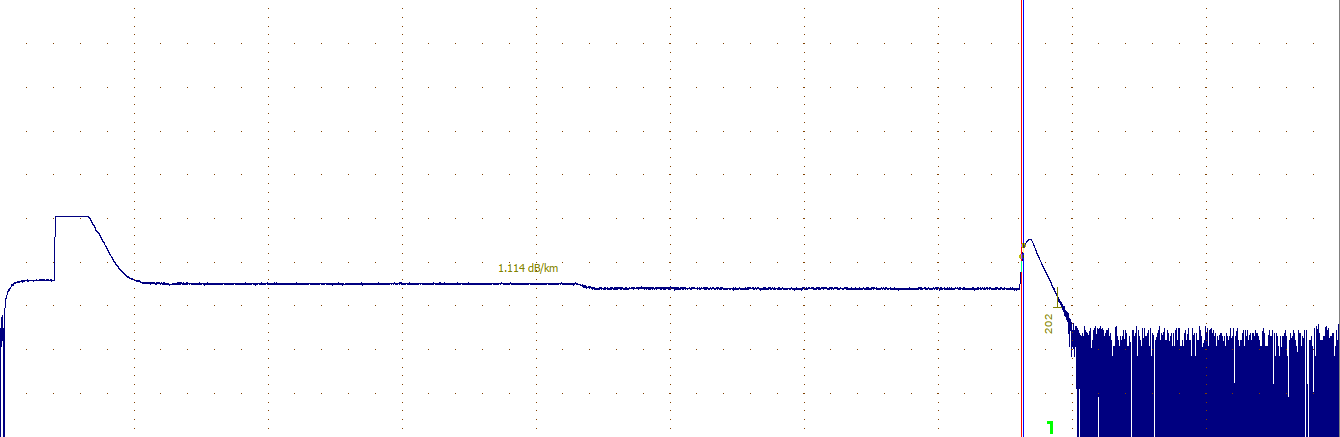
\includegraphics[width=0.5\linewidth]{images/Bab_4/Bab_4_3g1}
			\caption[Trace SM-MMFSI-SM ]{\small{Hasil trace OTDR pada baik SM-MMFSI-SM normal maupun SM- MMFSI dengan gangguan}}
		\end{figure}
	
		Sebagai acuan untuk mengetahui adanya interferensi pada serat optik multimode, diukur transmition antara sebelum dan sesudah bending. 
		Pengukuran menggunakan Fiber Tester dan OPM JW3208 pada panjang gelombang yang sama dengan trace OTDR yaitu 1550 nm.
		Hasil sementara menunjukkan bahwa terjadi selisih transmition pada nilai stabil 50 nW pada bending menurut setup di atas.
		Namun tidak terjadi perubahan pada trace OTDR baik sebelum atau sesudah bending. 
	
	\end{enumerate}

%=============================================================================
\newpage
	\subsection{Uji Gangguan Pagar}
	
	Dengan memperhatikan setiap hasil uji perlakukan sebelumnya, maka selanjutnya dilakukan uji eksperimen dengan kawat sebagai pengganti pagar. 
	Konfigurasi yang dipilih adalah Singlemode-Multimode-Singlemode.
	Setup yang dilakukan adalah dengan membentangkan kawat yang disatukan dengan serat optik, kemudian dilakukan uji \textit{bending} atau \textit{displacement}.\cite{Tian2017}\cite{Gong2011}\cite{Arifin2015} 
	Panjang yang digunakan adalah 1 meter dan 5 meter mengingat standar panjang unit pagar adalah 2,4 meter.\cite{Pagar2015}
	
	Berikut adalah setup pengujian:
	
	\begin{figure}[h!]
		\centering
		\captionsetup{justification=centering}
		\begin{subfigure}[b]{0.3\textwidth}
			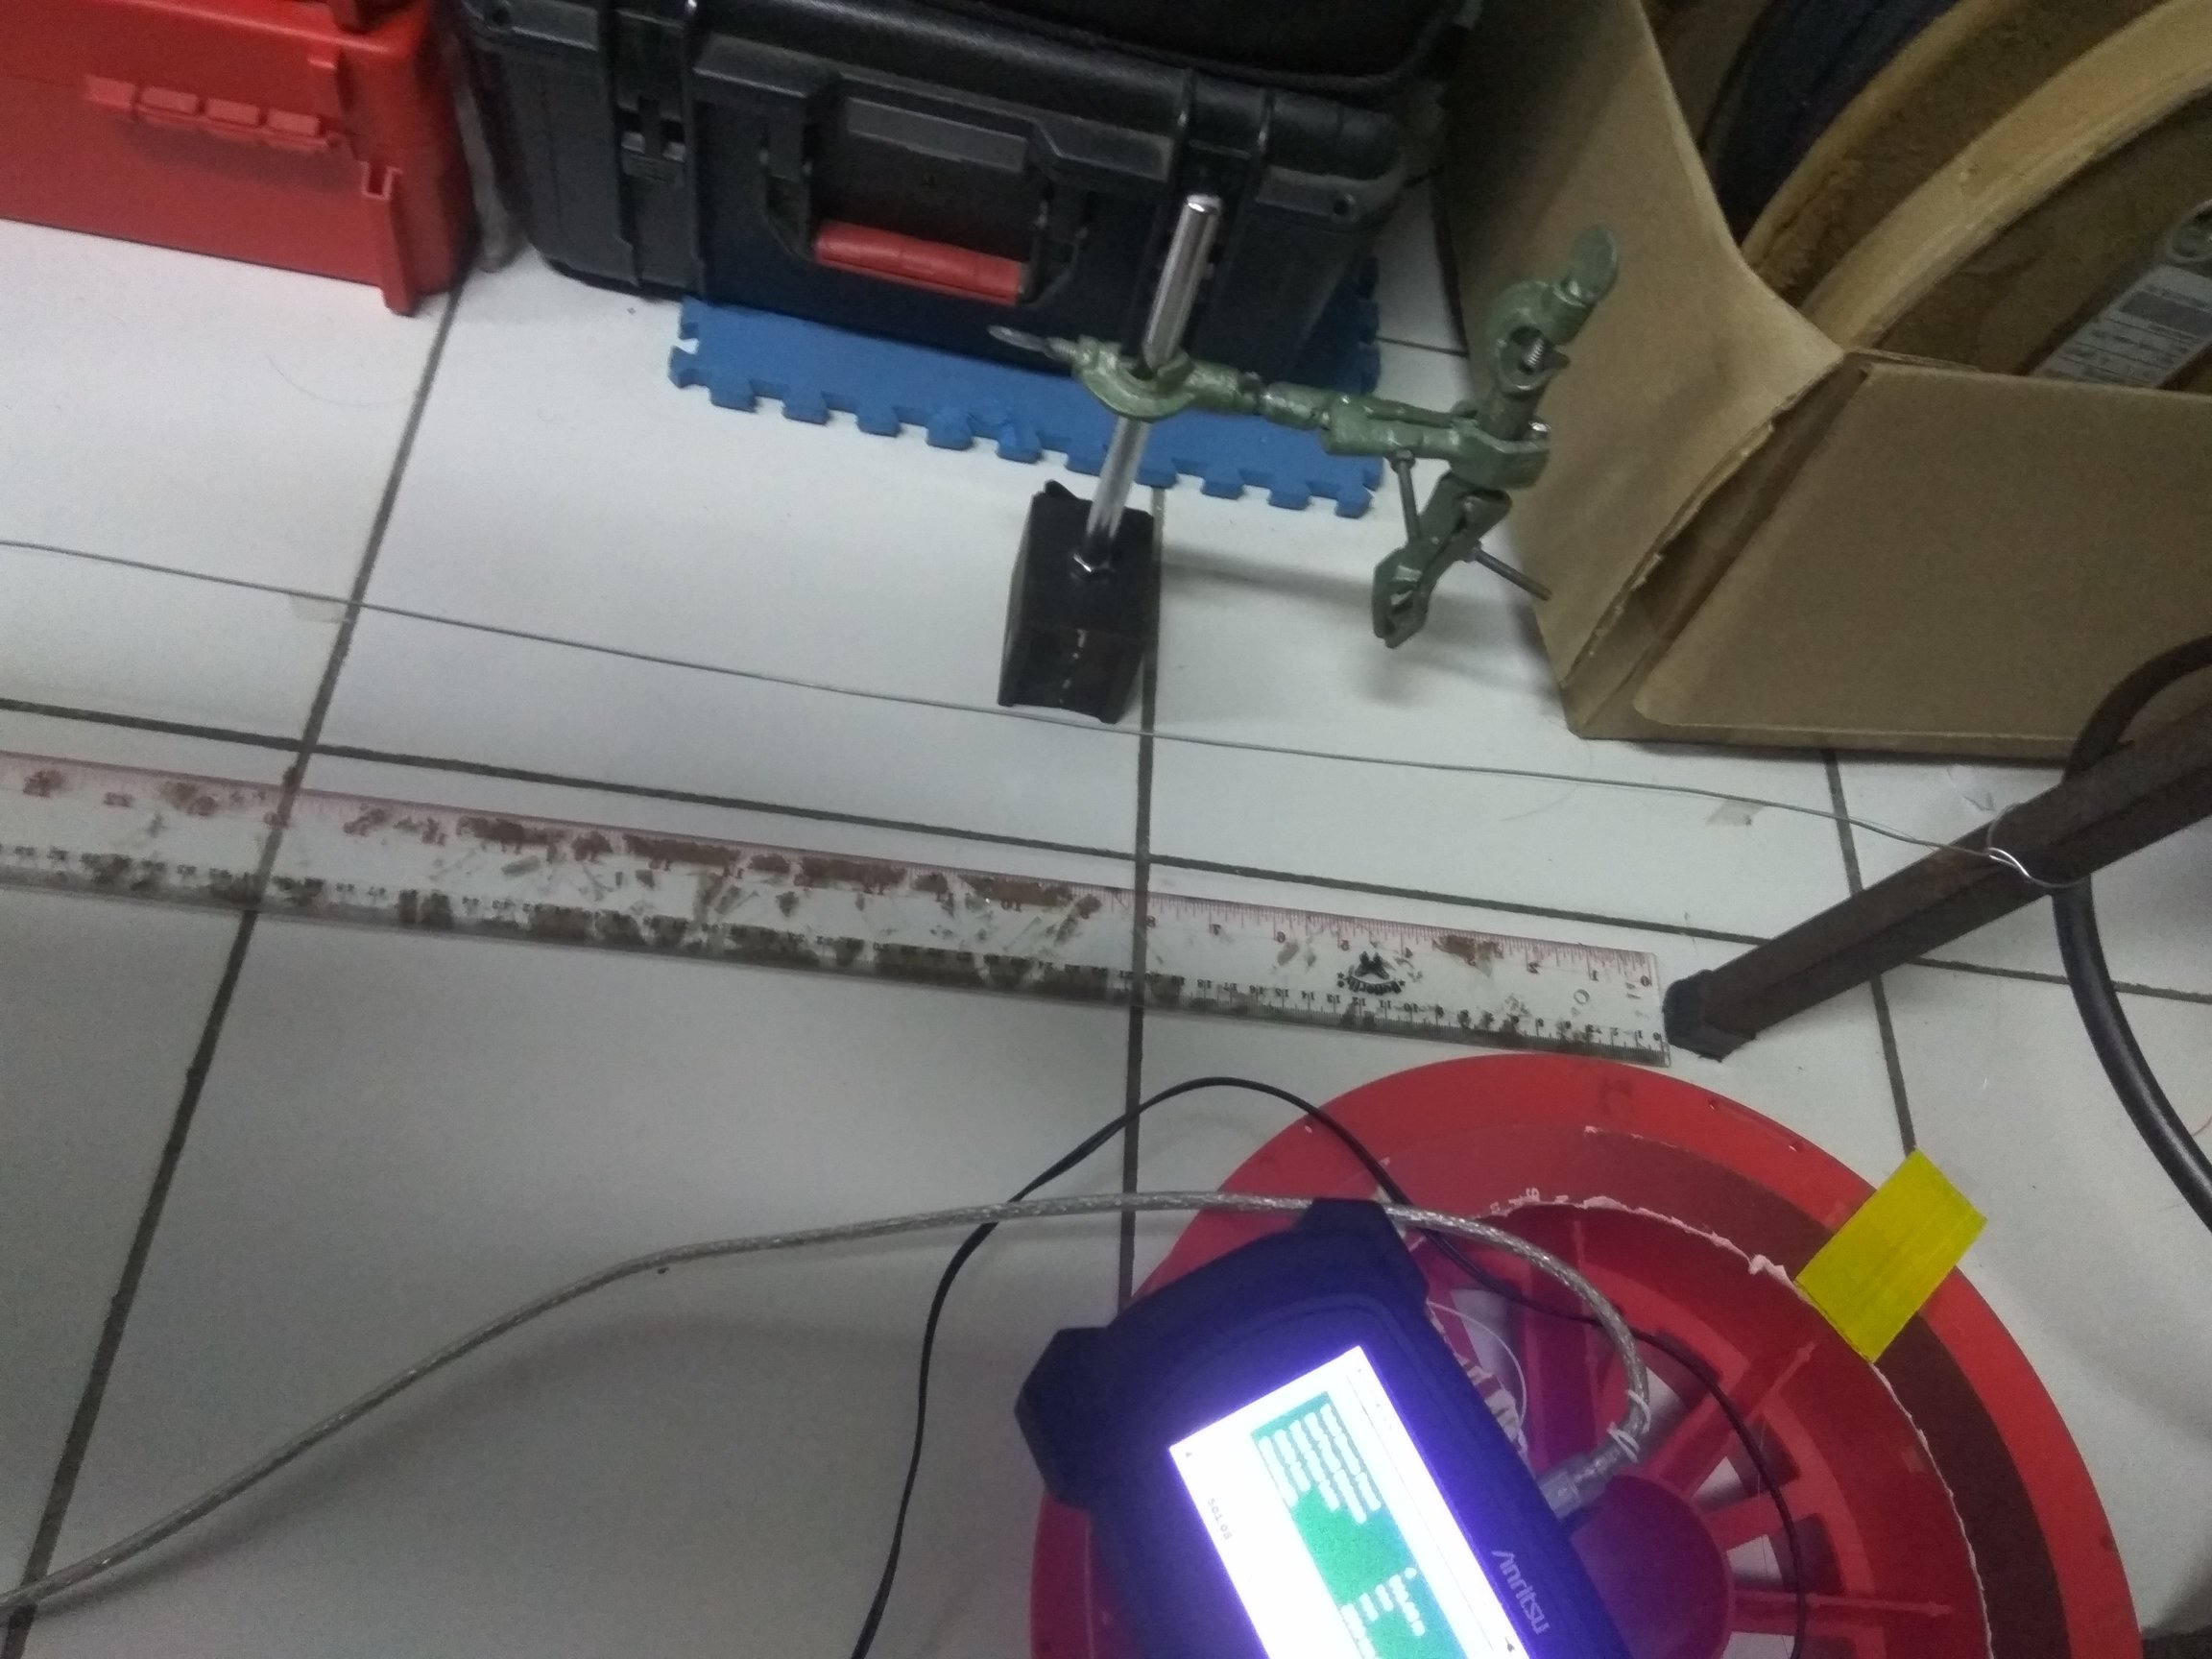
\includegraphics[width=\textwidth]{images/Bab_4/Bab_4_5a}	
			\caption{\small{Ujung awal dan OTDR}}		
		\end{subfigure}
		\begin{subfigure}[b]{0.3\textwidth}
			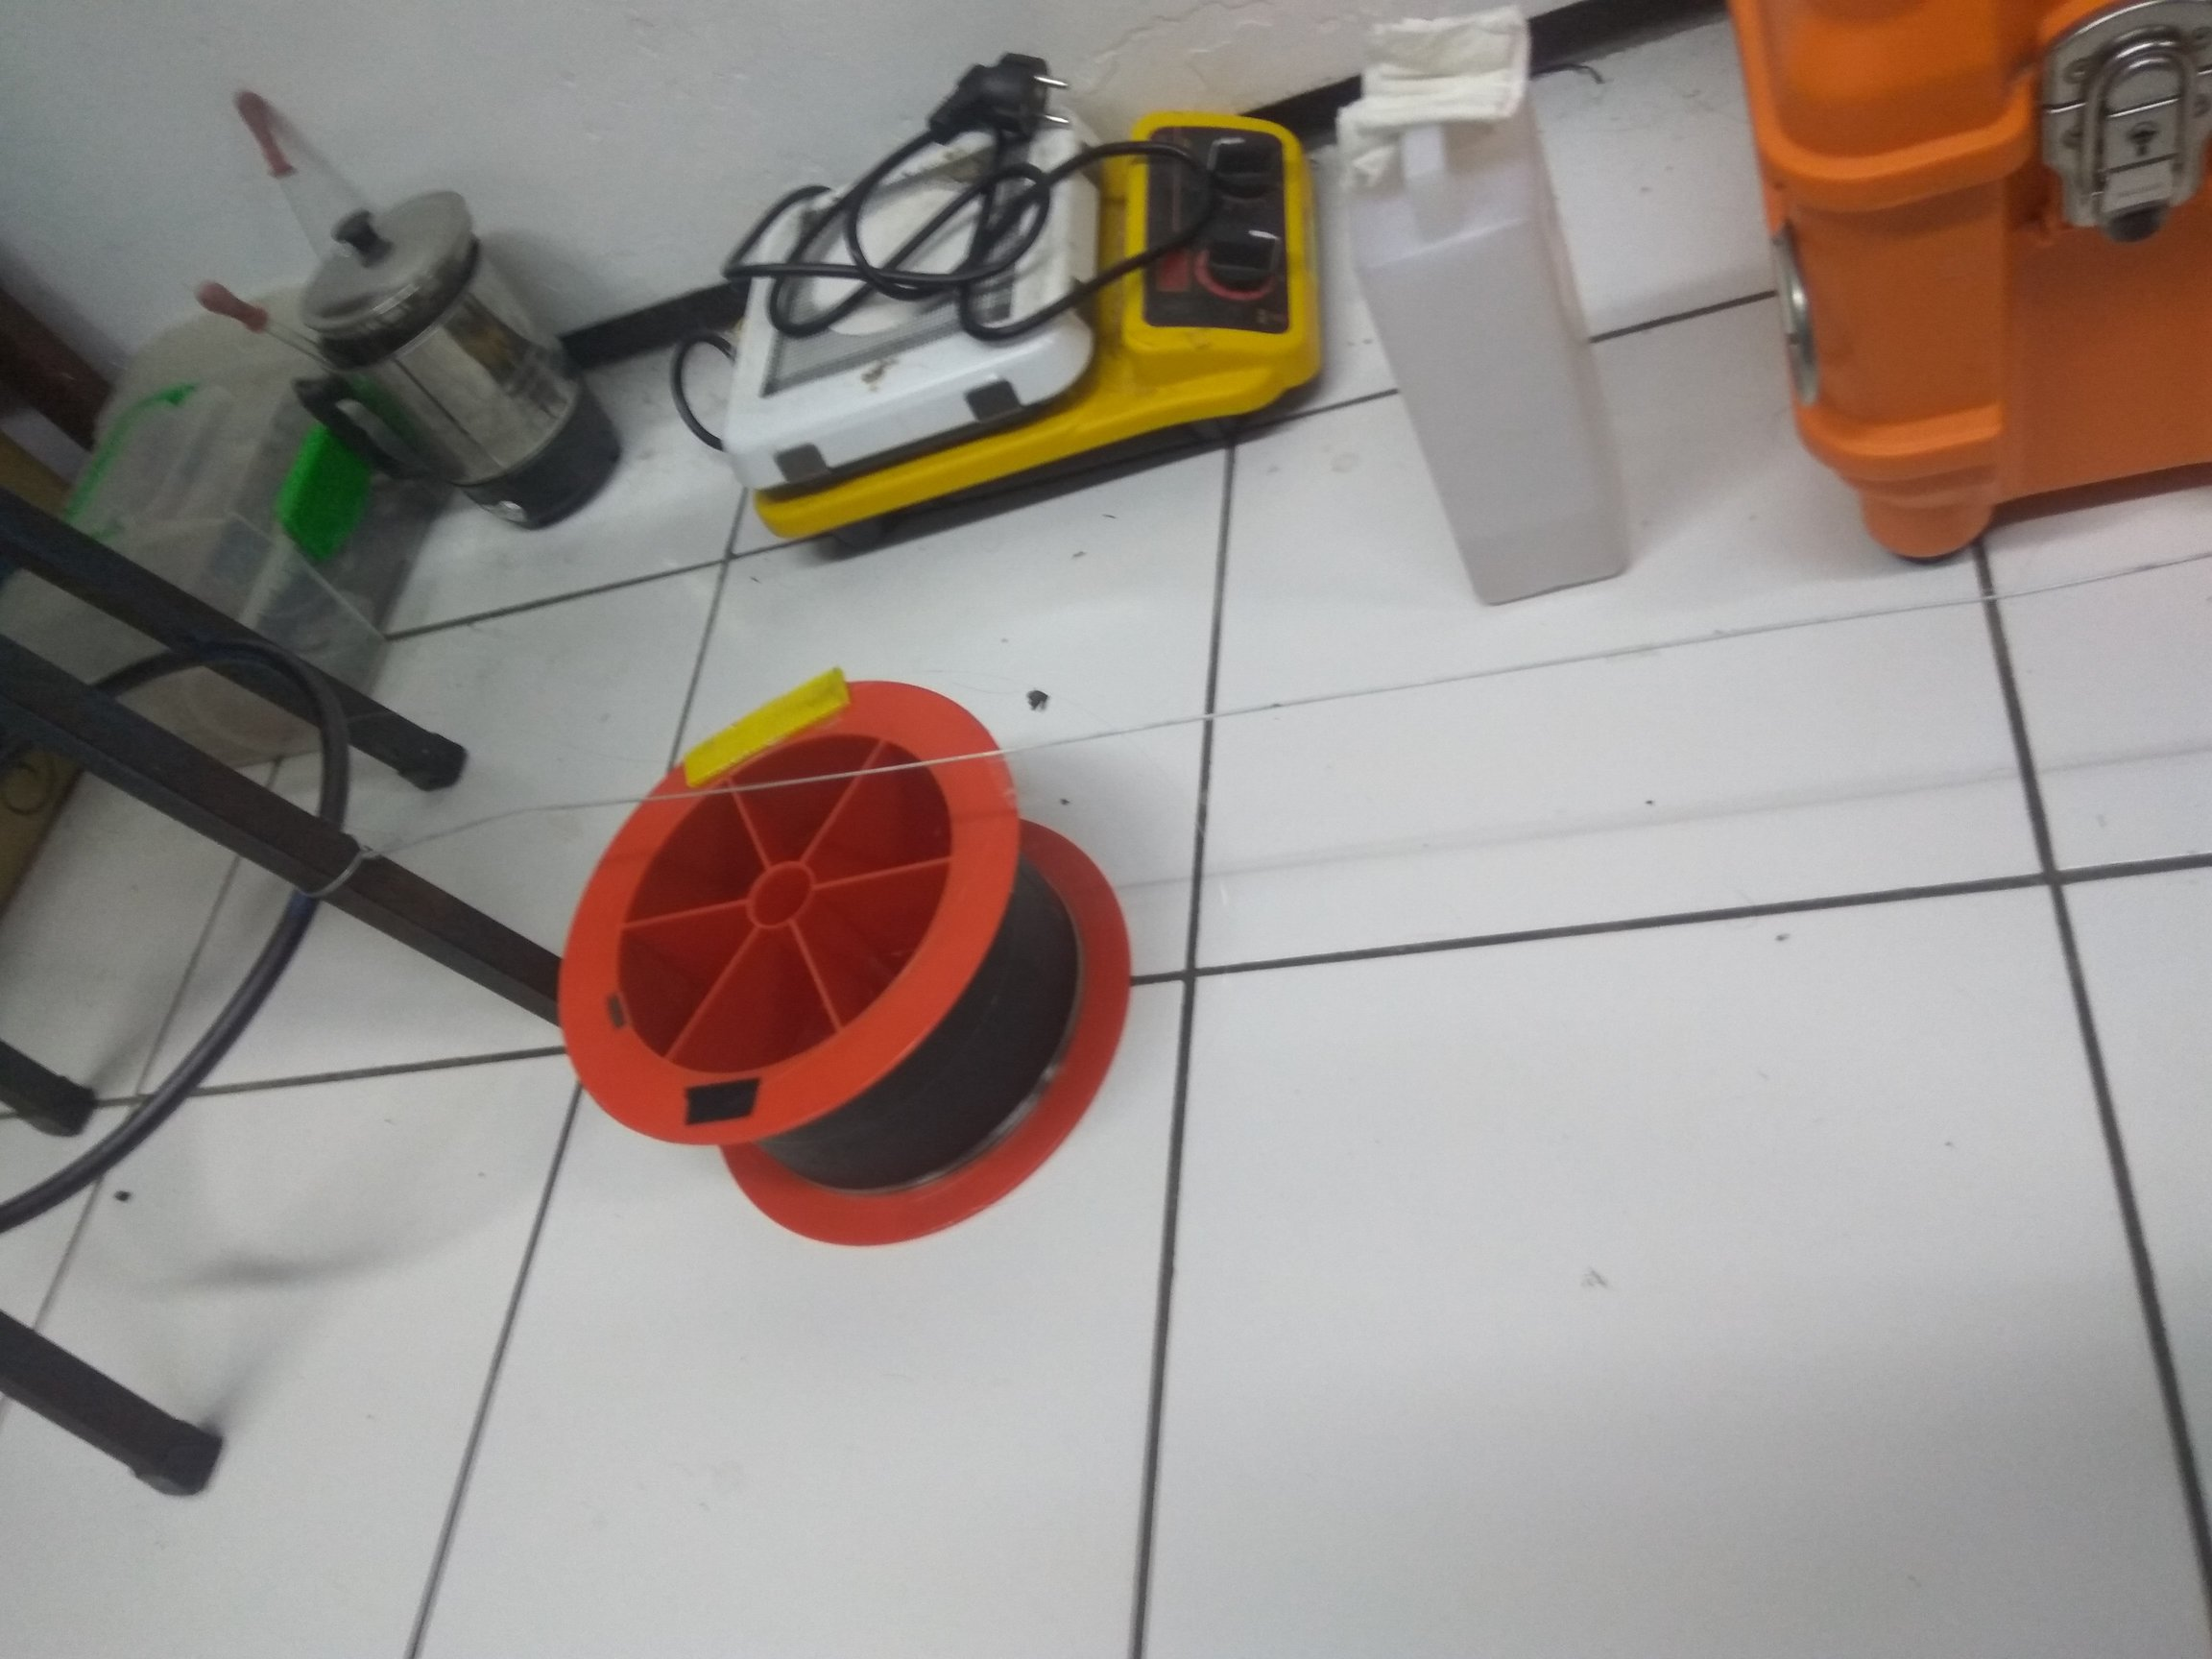
\includegraphics[width=\linewidth]{images/Bab_4/Bab_4_5b}
			\caption{\small{Ujung akhir}}			
		\end{subfigure}
		\begin{subfigure}[b]{0.4\textwidth}
			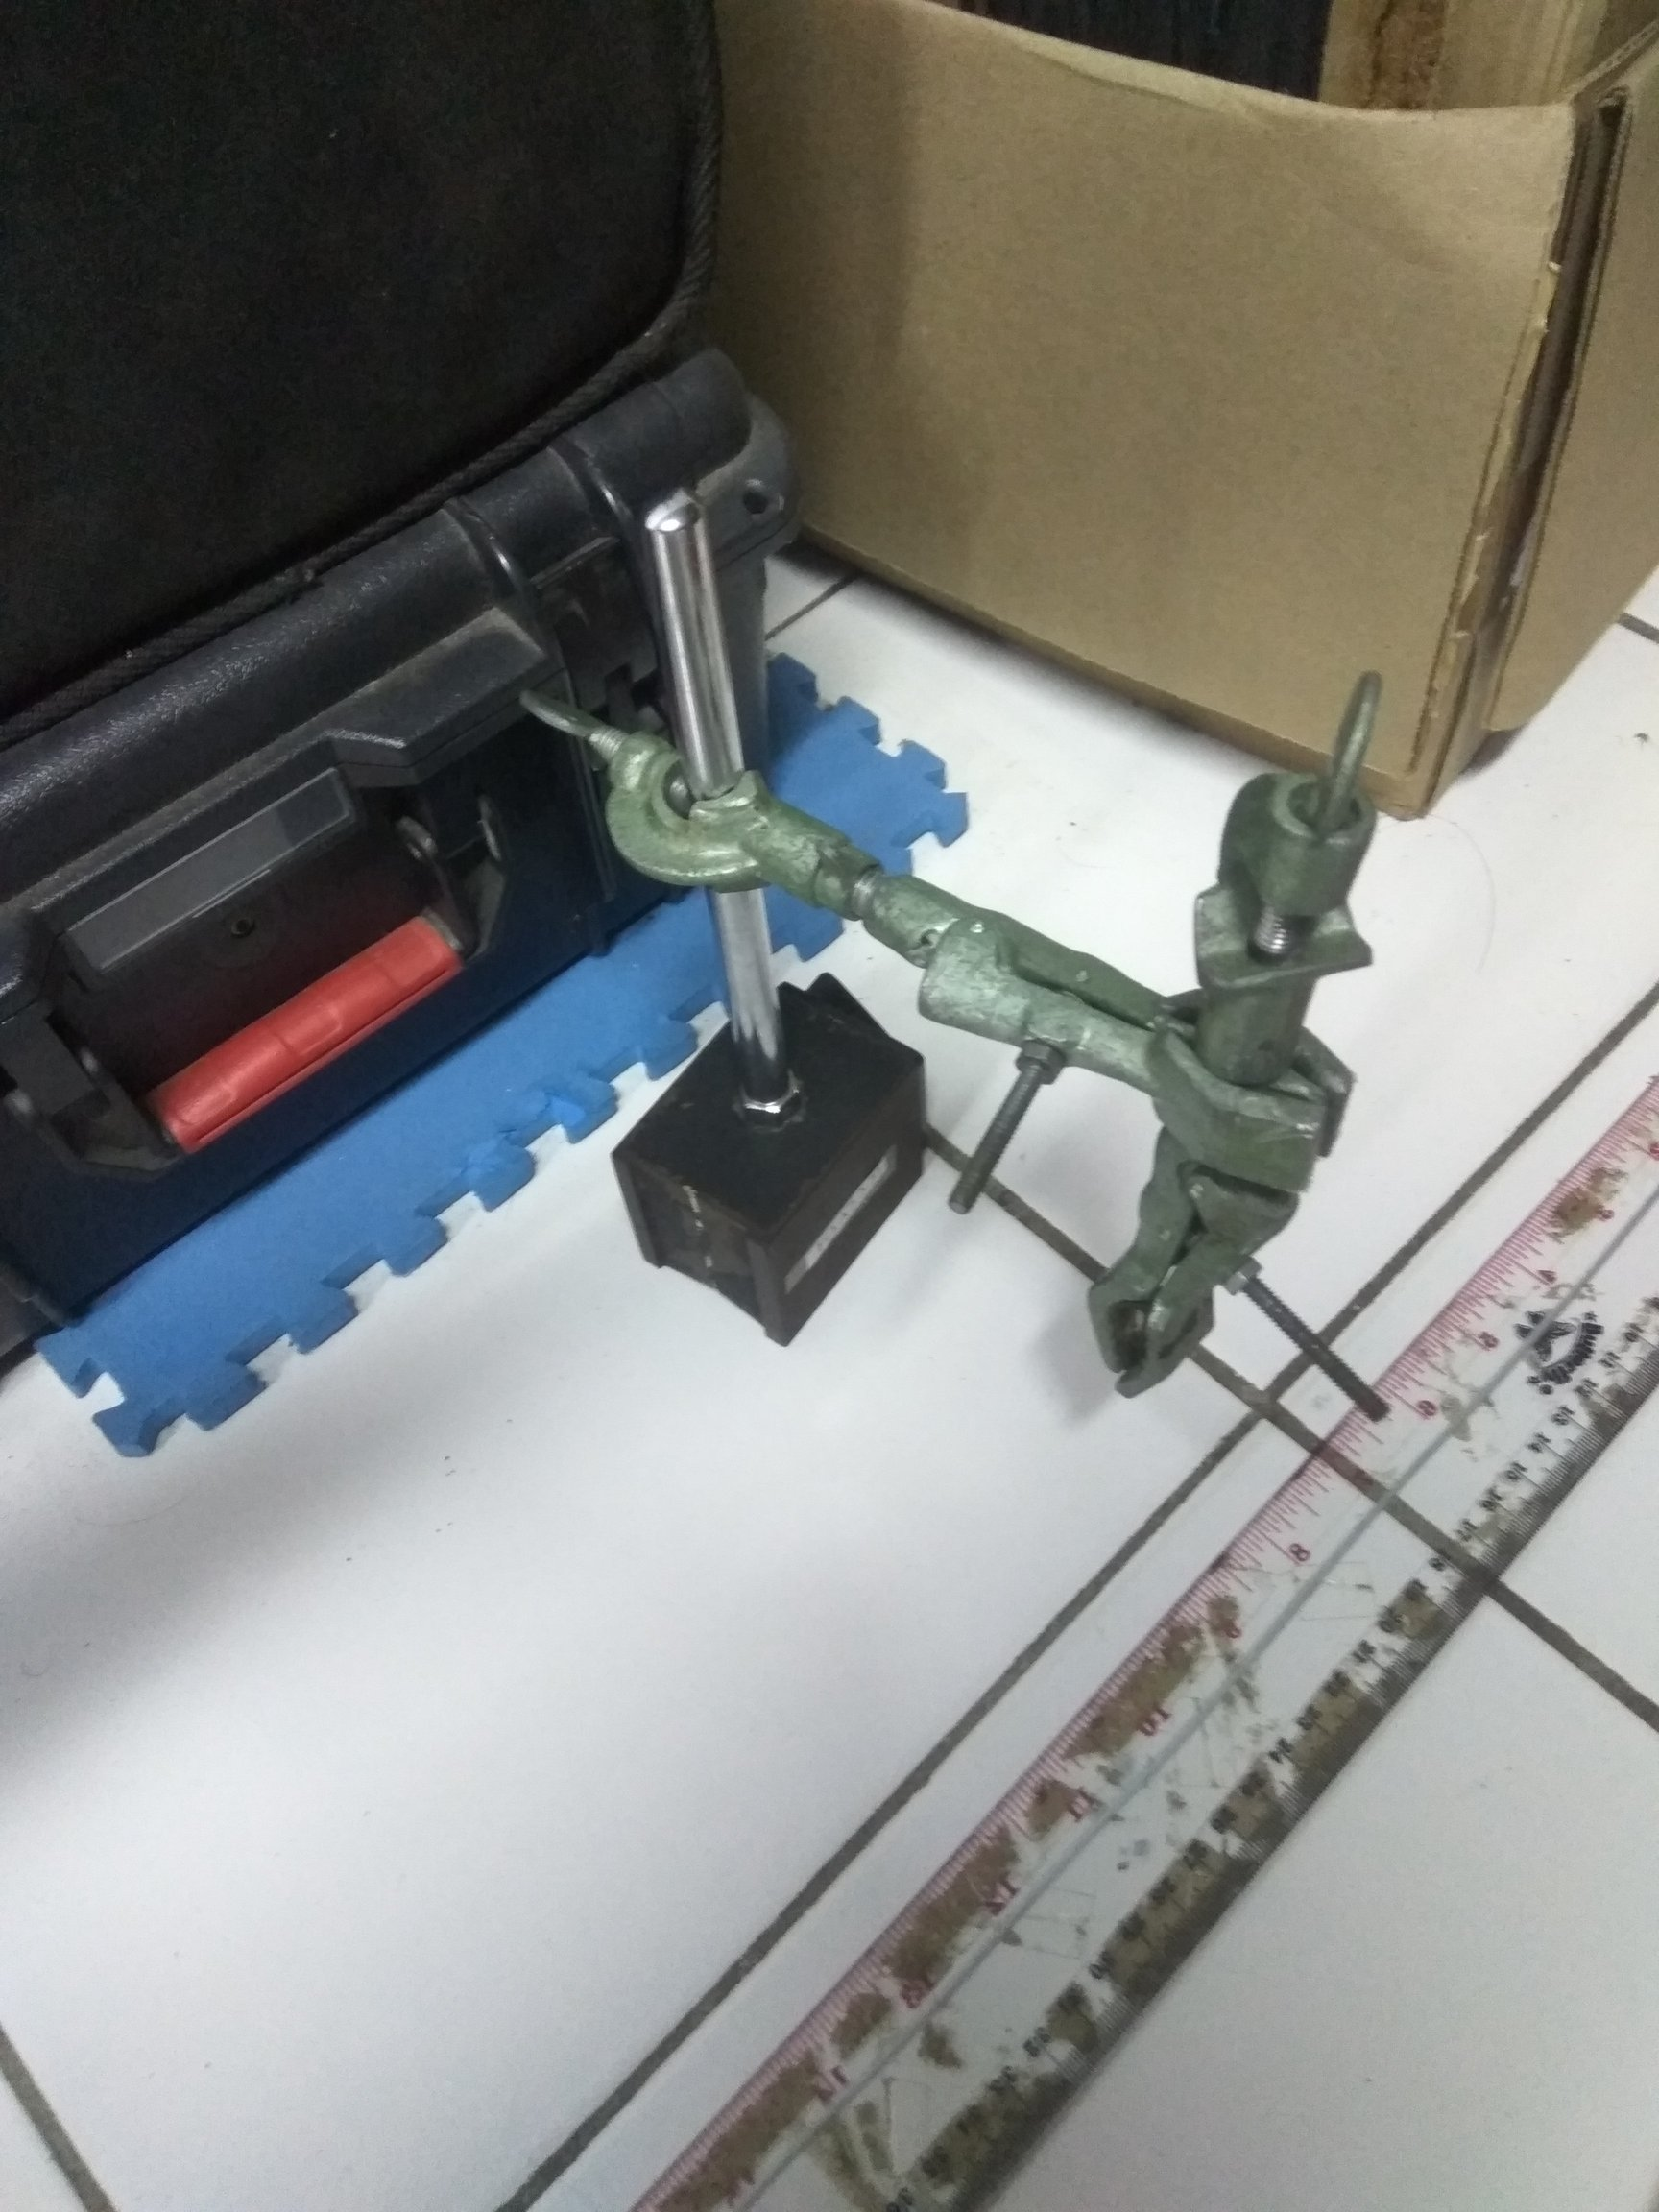
\includegraphics[width=\linewidth]{images/Bab_4/Bab_4_5c}
			\caption{\small{Statif dan holder untuk \textit{bending/displacement}}}			
		\end{subfigure}
		\caption[Uji Pagar]{\small{Gambaran Uji Gangguan Pagar }}
	\end{figure}

	Sedangkan \textit{displacement} yang dilakukan adalah sejauh 5mm, 10mm, 15mm, 20mm, dan 25mm vertikal ke bawah.
	Nilai yang diperhatikan adalah nilai puncak pada dua event, yaitu
	
	\begin{itemize}
		\item fiber \textit{splice}, yaitu \textit{splice} antara singlemode dan multimode  
		\item fiber \textit{splice}, yaitu \textit{splice} antara multimode dan singlemode.
		Splice kedua ini hanya muncul pada setup fiber 5 meter 
		\item fiber \textit{end}, yaitu ujung akhir fiber singlemode terakhir.
	\end{itemize}

	Sedangkan posisi displacement adalah setiap penambahan jarak konstan 20cm.
	
	Grafik hasil secara umum di semua pengujian 1 meter adalah sebagai berikut:
	
	\begin{figure}[h!]
		\centering
		\captionsetup{justification=centering}
		\begin{subfigure}[b]{0.7\textwidth}
			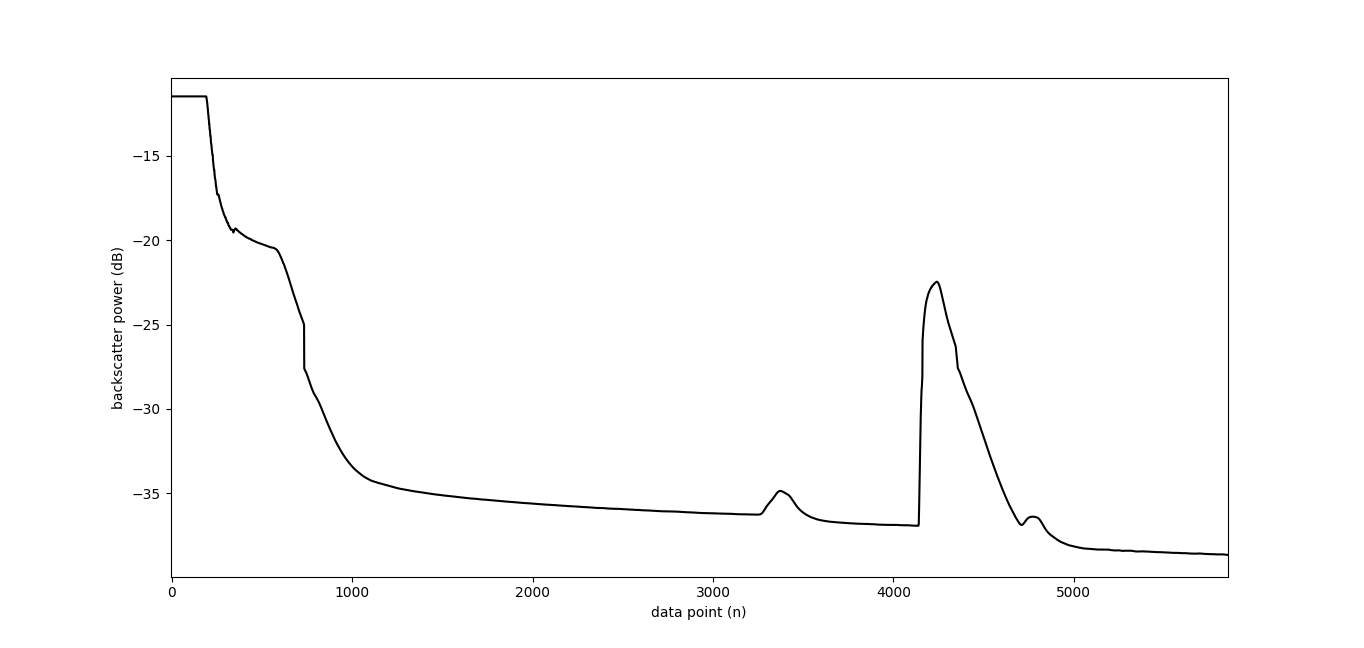
\includegraphics[width=\textwidth]{images/Bab_4/Bab_4_5d1}	
			\caption{\small{Grafik trace dasar}}		
		\end{subfigure}
		\begin{subfigure}[b]{0.7\textwidth}
			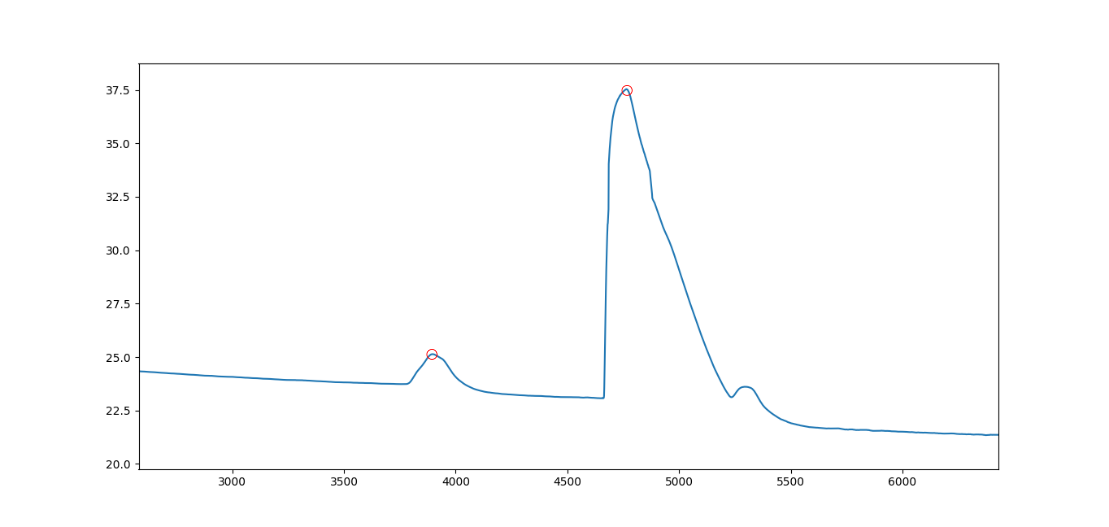
\includegraphics[width=\linewidth]{images/Bab_4/Bab_4_5d2}
			\caption{\small{Nilai puncak event fiber \textit{Splice} dan \textit{End}}}			
		\end{subfigure}
		\caption[Uji Pagar]{\small{Grafik hasil Trace untuk panjang 1 meter}}
	\end{figure}

	Grafik hasil secara umum di semua pengujian 5 meter adalah sebagai berikut:
	
	\begin{figure}[h!]
		\centering
		\captionsetup{justification=centering}
		\begin{subfigure}[b]{0.7\textwidth}
			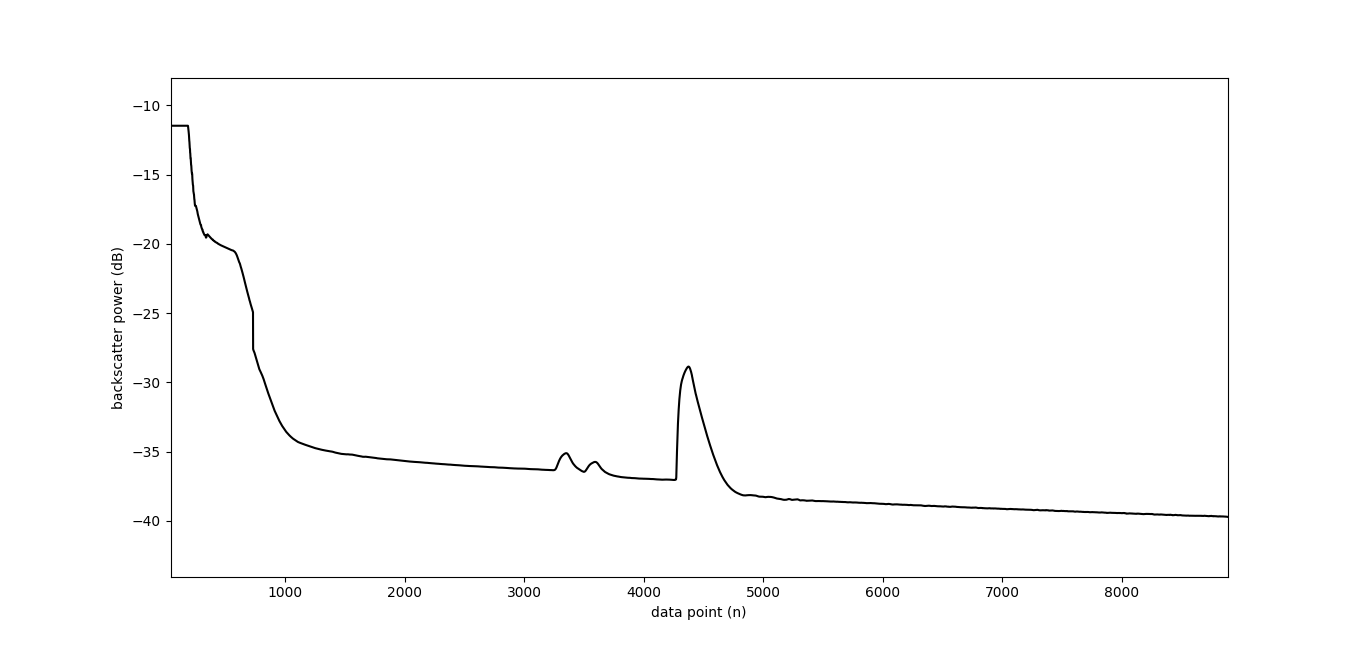
\includegraphics[width=\textwidth]{images/Bab_4/Bab_4_5e1}	
			\caption{\small{Grafik trace dasar}}		
		\end{subfigure}
		\begin{subfigure}[b]{0.7\textwidth}
			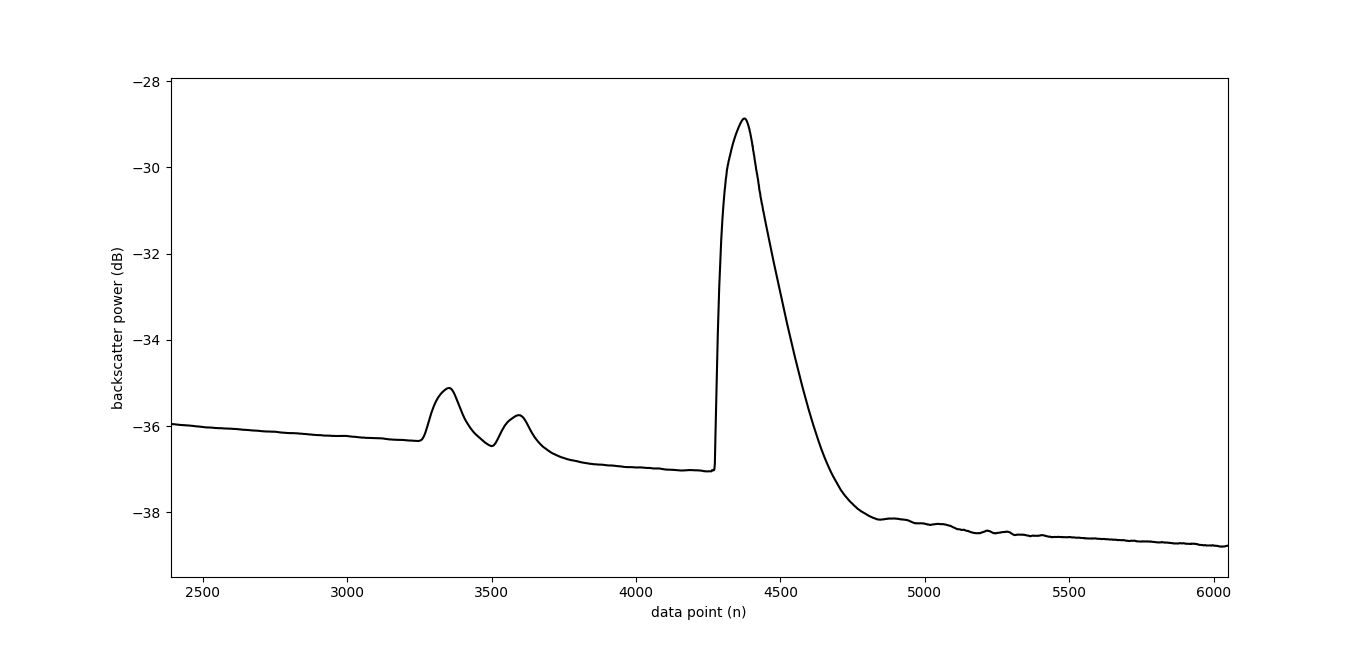
\includegraphics[width=\linewidth]{images/Bab_4/Bab_4_5e2}
			\caption{\small{Nilai puncak event fiber \textit{Splice} dan \textit{End}}}			
		\end{subfigure}
		\caption[Uji Pagar]{\small{Grafik hasil Trace untuk panjang 5 meter}}
	\end{figure}

%=============================================================================
\newpage

	Selanjutnya, didapatkan selisih semua nilai puncak event terhadap kondisi tanpa gangguan,
	sehingga dapat ditemukan respon fiber di setiap posisi dan ukuran \textit{displacement}.
	Berikut adalah grafik respon pada event \textit{splice} dan \textit{end}.
	
	\begin{figure}[h!]
		\centering
		\captionsetup{justification=centering}
		\begin{subfigure}[b]{0.6\textwidth}
			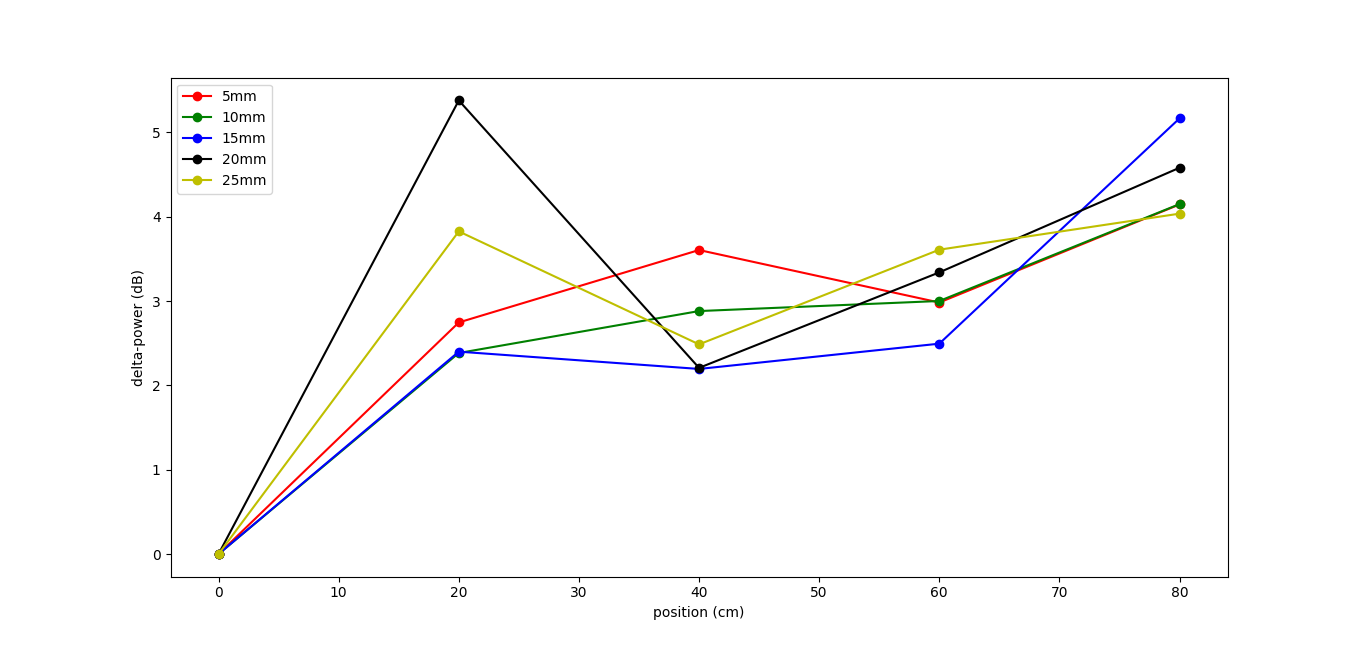
\includegraphics[width=\textwidth]{images/Bab_4/Bab_4_5f1}	
			\caption{\small{Respon fiber end}}		
		\end{subfigure}
		\begin{subfigure}[b]{0.6\textwidth}
			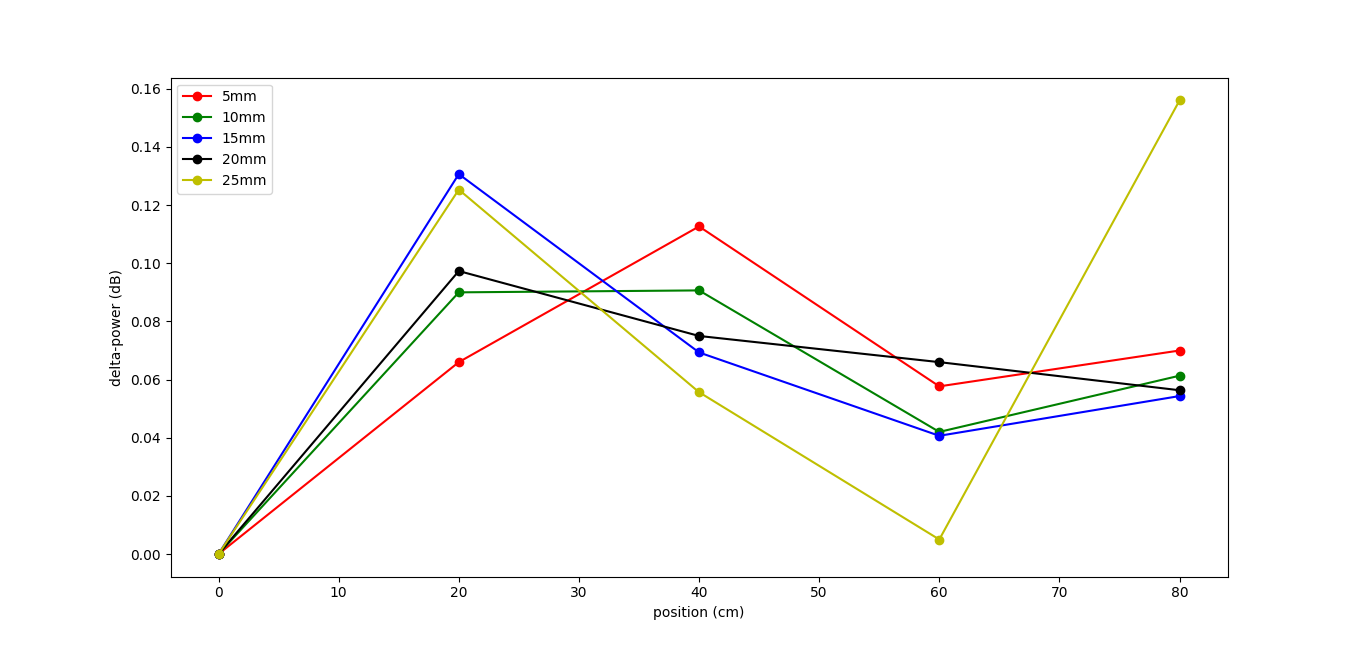
\includegraphics[width=\linewidth]{images/Bab_4/Bab_4_5f2}
			\caption{\small{Respon fiber splice}}			
		\end{subfigure}
		\caption[Uji Pagar]{\small{Respon selisih terhadap kondisi normal pada 1 meter}}
	\end{figure}

	Selanjutnya untuk grafik 5 meter adalah sebagai berikut:
	
	\begin{figure}[h!]
		\centering
		\captionsetup{justification=centering}
		\begin{subfigure}[b]{0.6\textwidth}
			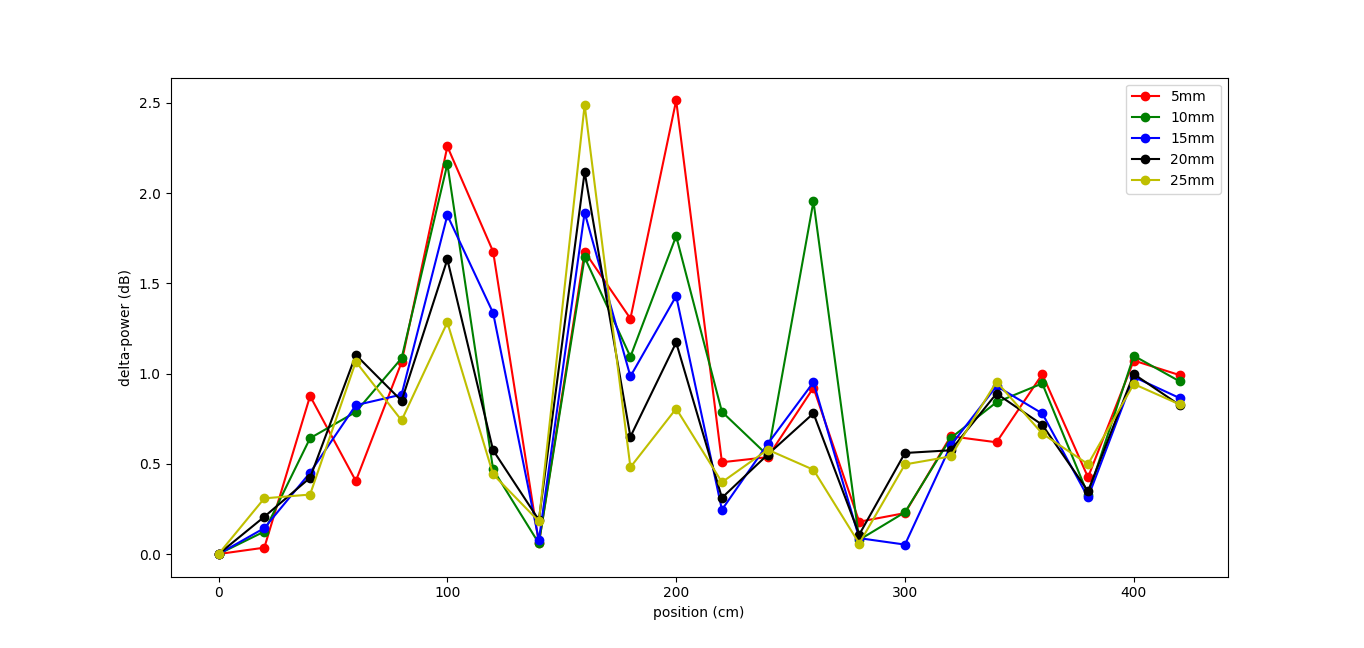
\includegraphics[width=\textwidth]{images/Bab_4/Bab_4_5g1}	
			\caption{\small{Respon fiber end}}		
		\end{subfigure}
		\begin{subfigure}[b]{0.6\textwidth}
			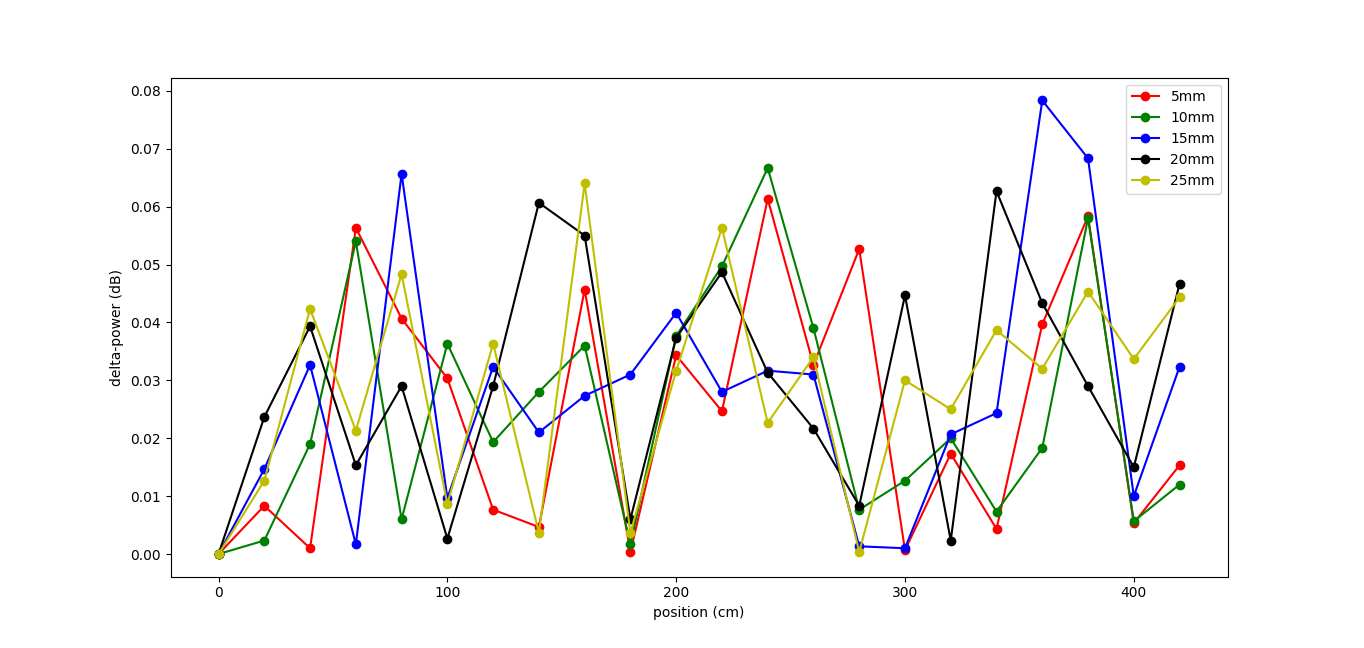
\includegraphics[width=\linewidth]{images/Bab_4/Bab_4_5g2}
			\caption{\small{Respon fiber splice 1 dan 2}}			
		\end{subfigure}
		\caption[Uji Pagar]{\small{Respon selisih terhadap kondisi normal pada 5 meter}}
	\end{figure}

%=============================================================================
% Daftar Pustaka

\newpage

	\section{Daftar Pustaka}
	
	\begin{center}
		\textbf{Daftar Pustaka}
	\end{center}
	
	\bibliographystyle{IEEEtran}
	\bibliography{/home/achmadi/Documents/BibTex/library.bib}
	%\bibliography{/home/fotoniks/Mendeley_BibTex/library.bib}

	
\end{document}
